\ifsvnmulti
 \svnkwsave{$RepoFile: lyapunov/KS.tex $}
 \svnidlong {$HeadURL$}
 {$LastChangedDate$}
 {$LastChangedRevision$} {$LastChangedBy$}
 \svnid{$Id$}
\fi

\chapter{\KS}
\label{sect:LyapKS}

This section of the blog deals specifically with the
\KS\ calculations. General discussion is entered into
\refchap{c-DailyBlog} {Daily blog}.

% PC 2011-03-02: (b) generated by Kazz kaz2-PhysModes-b.png
\begin{figure}
 (a)~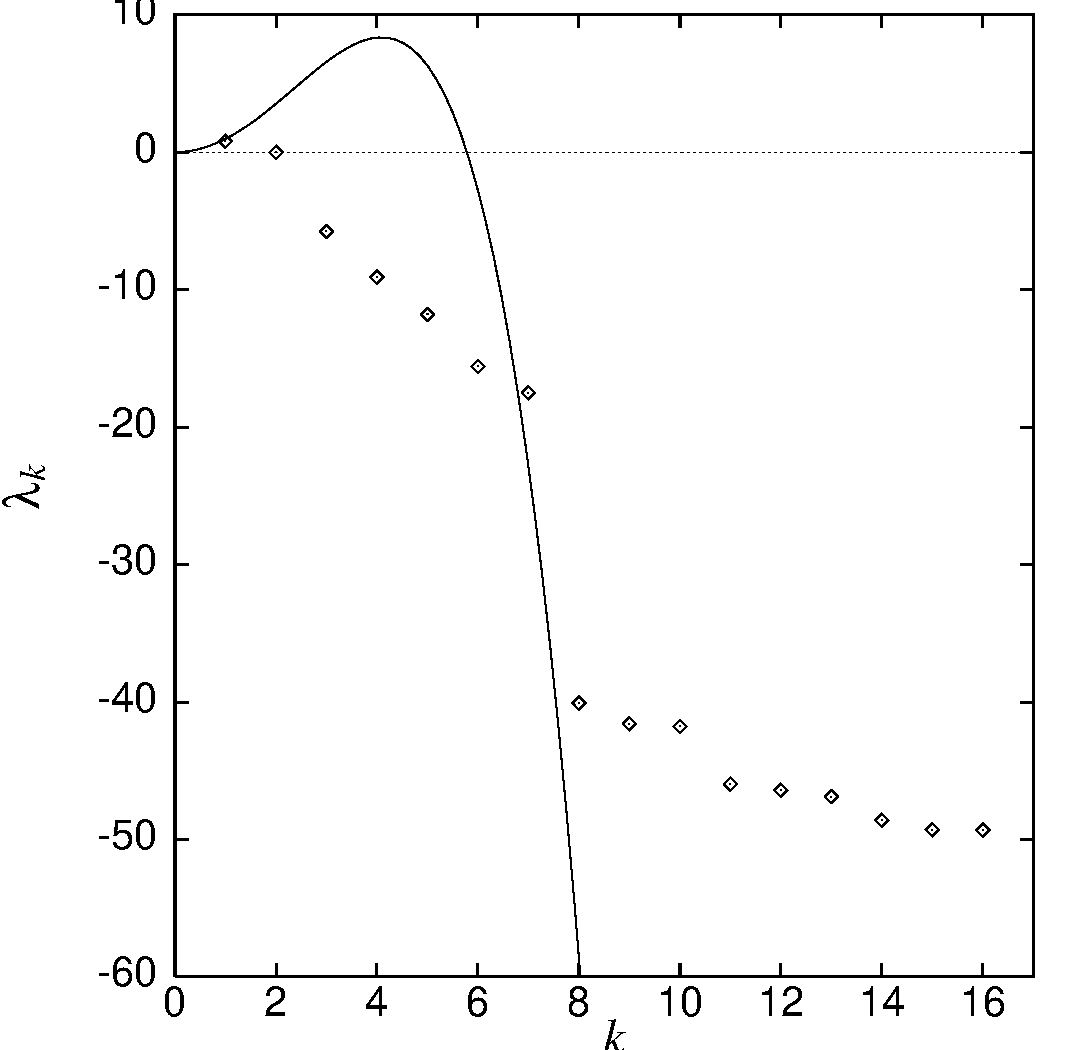
\includegraphics[width=0.40\textwidth]{eigenvalues}
 (b)~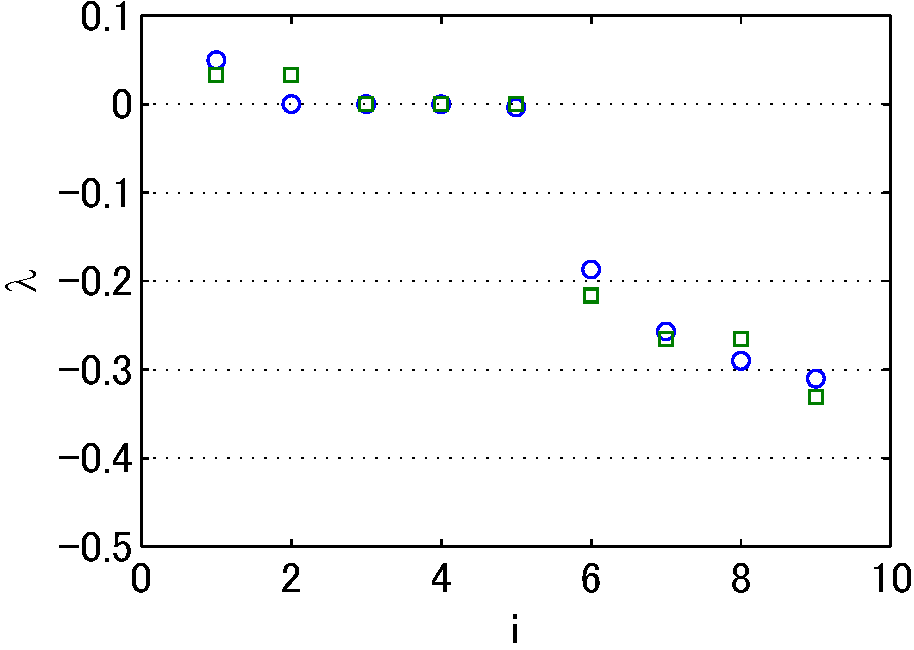
\includegraphics[width=0.50\textwidth]{kaz2-PhysModes-b}
\caption{
(a)
Lyapunov exponents $\lambda_k$ versus $k$ for the periodic
orbit $\overline{1}$ compared with  the stability eigenvalues
of the $u(x,t)=0$ stationary solution $k^2- \nu k^4$ (from
\refref{Christiansen97}). $\lambda_k$ for $k \geq 8$ fall
below the numerical accuracy of integration and are not
meaningful. Antisymmetric subspace,
hence no \SOn{2}\ pairing of eigenvalues, $N=16$ real Fourier
modes, $L=36.31$. One needs to rescale the time to compare
this to figure (b); -60 in the Lyapunov scale of figure (a)
corresponds to approx. -1.8 in \reffig{fig:lyapSpec}\,(a).
(b)
First 9 Lyapunov exponents $\lambda_j$ for the full
\statesp, periodic b.c. KS for $L=22$, from a 124 real Fourier
modes (blue circles) long-time simulation overlayed on
the \po\ \PO{10.25} (green squares) [Kazz 2011-02-21].
}
\label{fig:lyapSpec1}
\end{figure}

% PC 2009-09-12: (a) generated by siminos/figSrc/gnu/lyapSpec.gnu
% PC 2011-03-02: (b) generated by Kazz kaz2-PhysModes-a.png
\begin{figure}
 (a)~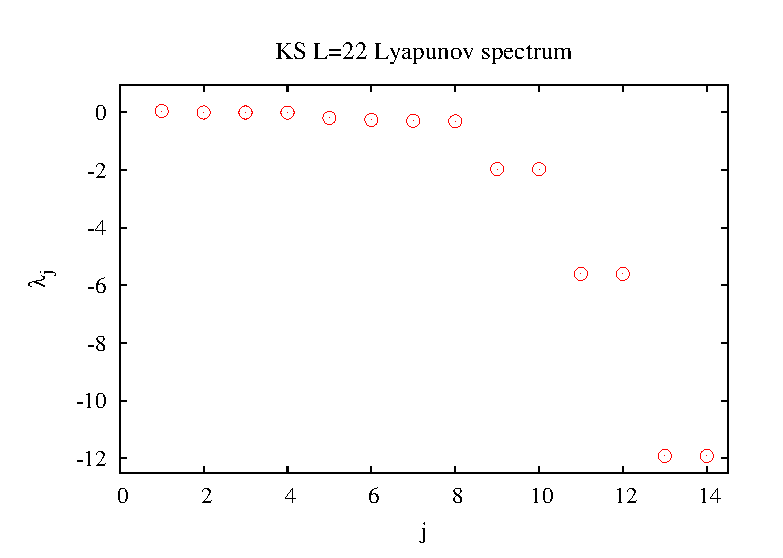
\includegraphics[width=0.48\textwidth]{lyapSpec}
 (b)~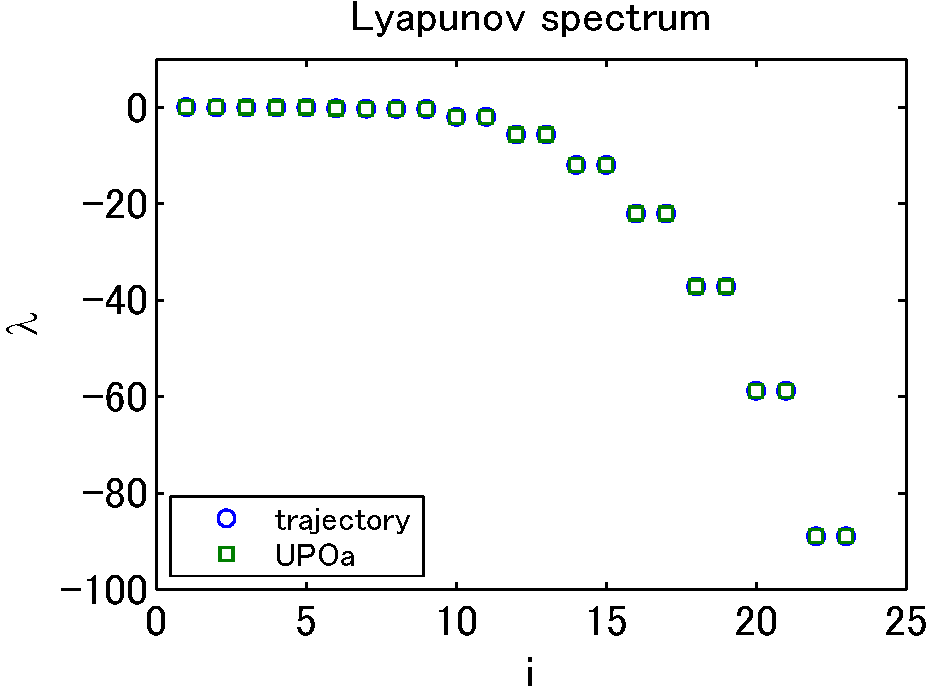
\includegraphics[width=0.42\textwidth]{kaz2-PhysModes-a}
\caption{
(a)
First 14 Lyapunov exponents $\lambda_j$ for the full
\statesp, periodic b.c. KS for $L=22$, from a 62 real Fourier
modes long-time simulation (from \refref{SCD07}).
(b)
First 24 Lyapunov exponents $\lambda_j$ for the full
\statesp, periodic b.c. KS for $L=22$, from a 124 real Fourier
modes (blue circles) long-time simulation overlayed on
the \po\ \PO{10.25} (green squares) [Kazz 2011-02-21].
}
\label{fig:lyapSpec}
\end{figure}

\begin{description}
\item[2009-09-13 Predrag]
Sure looks persuasive, see \reffig{fig:lyapSpec}. I have also
added stability of a periodic orbit from
\refref{Christiansen97}, for KS on the periodic b.c.,
antisymmetric subspace, system size $\tilde{L} = 5.8$ close
to the onset of chaos, 16 real Fourier modes. As (perhaps?)
discussed in \refref{lanCvit07}, one has to be careful about
defining the effective system size $\tilde{L}$ for the
antisymmetric subspace, so these computations are done on
$L=36.31$ (or $L = 18.155$ if one considers the fundamental
$[0,L/2]$ domain only). Going from $(L,\nu) =
(2\pi,0.029924)$ of \refref{Christiansen97} to $(L,\nu) =
(L,1)$ convention used here requires that the time be
rescaled as $t \to \nu t$, and the Lyapunov exponents as
$\lambda_i \to \lambda_i/ \nu = \lambda_i/ 0.029924 $, so -60
in the Lyapunov scale of \reffig{fig:lyapSpec}\,(a)
corresponds to approx. -1.8 on the scale of
\reffig{fig:lyapSpec}\,(b), which would mean that then we
computed only the first pair of isolated eigenvalues. The
reason is that for periodic orbits we are computing {\em
Floquet multipliers} which underflow numerically very
quickly, so we cannot compute many {\em Floquet exponents}.
These covariant Lyapunov eigenvector methods are apparently
much smarter.

In \refref{lanCvit07} computations are done at $L = 38.5$,
but we listed only 4 eigenvalues per periodic orbit, and
considering hopeless organizational skills on the Lan astral
plane, I doubt that the full spectra can be rescued from
Lan's calculations. And, as explained above, probably we cannot
compute them for periodic orbits.

\item[2009-09-13 Ruslan]
 Here's the expanded list of Lyapunov exponents for KS with $L = 22$:
 0.048,    0.0,    0.0,   -0.003,   -0.189,   -0.256,   -0.290,   -0.310,
-1.963,   -1.967,   -5.605,   -5.605,  -11.923,  -11.923...
So, there appears to be 8 `physically relevant' exponents and
the rest are pairs of hyperbolically separated ones.

I read
the papers about these covariant Lyapunov vectors and I'm not
sure I understand how they are related to eigenvectors at
periodic orbits: are they aligned?  I suspect that not quite,
apart from the most expanding and the most contracting
direction, the rest are sitting somewhere within the
subspaces spanned by the $k$ most expanding, or $m$ most
contracting eigendirections, but not quite aligned with the
eigendirections themselves.  That's probably why they are
more appropriately called `Lyapunov vectors'.

\item[2009-09-14 Predrag]
The `covariant Lyapunov vectors' are indeed the (right,
non-orthogonal) eigenvectors of the \jacobianM\ \jMps, as
defined in ChaosBook, and coincide with Floquet eigenvectors
for a periodic orbit.

 \item[Ruslan] I use 32 complex Fourier modes, so the
truncated system has 62 degrees of freedom.  The Lyapunov
exponent calculation is standard (using Gram-Schmidt).  The
exponents are the same, independent of the method of
calculation.  I have not attempted to calculate the covariant
Lyapunov vectors. I'm pretty sure that
orthogonality between physical and isolated eigenvectors
applies, but have not checked.

 \item[Ruslan]
It's OK to I email Hong-liu
Yang\rf{YaTaGiChRa08}, ask him to rerun his covariant
Lyapunov vector spectrum for $L=22$, to see whether he agrees
with us.

 \item[Ruslan]
I have the 62 eigenvalues/eigenvectors for all the RPO/PPO
I've detected, but for the highly contracting eigenvalues
the straightforward calculation
suffers from the numerical noise. We need a
better method to compute Floquet multipliers. I have now
checked:   Looks like {Kurt Lust} has proposed one, but I
cannot get his paper on ``Improved Numerical Floquet
Multipliers''\rf{Lust01}. If you could
get it for me, it would be great.

\item[2009-09-13 Ruslan]
``Structure of characteristic Lyapunov
vectors in spatiotemporal chaos''\rf{PaSzLoRo09} states
that characteristic Lyapunov vectors ``reduce to the Floquet
eigenvectors for a periodic orbit'' and references Trevisan
and Pancotti\rf{TrePan98}, which I cannot get electronically.

\item[2009-09-14 Predrag]
I added abstracts of these papers to the reading list above.
The `covariant Lyapunov vectors' are indeed the (right,
non-orthogonal) eigenvectors of the \jacobianM\ \jMps, as
defined in ChaosBook, and coincide with Floquet eigenvectors
for a periodic orbit. For a flow they are defined at a given
\statesp\ point by going back and forward a finite, but
`sufficiently long' time $t$, and coincide with the Floquet
eigenvectors if the point is (relative) periodic. I believed
that for a PDE we cannot go backward, but was wrong; the do
it by using the segment of forward trajectory stored in
memory. The reason why one can get the Floquet {\em exponent}
for arbitrarily long orbit is that the multiplier for eigenvector
evolved in time is just a number, so taking its logarithm over
short time segments and
storing it is trivial, no underflow problems one would get if
one worked with the Floquet {\em multiplier}. So we should be able
to keep track of all 62 eigenvectors, redo it for 126 eigenvectors,
and compare with plots in \refref{YaTaGiChRa08}.
Ginelli \etal\rf{ginelli-2007-99} are the main
reference on the `covariant Lyapunov vectors.' They describe
the QR algorithm for computing Gram-Schmidt vectors (GSV) and
recovering the covariant Lyapunov vectors (CLV) from them.
What confuses me is that so far all papers refer to $\Lyap_j
= \eigRe_j + i \, \eigIm_j$ as purely real, and list only
$\eigRe_j$, but I guess that will be explained somewhere.

\item[2009-09-14 Predrag]
My initial \reffig{fig:lyapSpec} was not optimal; I have now
replotted it as in Fig.~4 of
Yang \etal\rf{YaTaGiChRa08},
agrees with their 'extensivity' plot for $L=96$ and $192$.

I prefer $x$-axis to be $j/\tildeL = 2 \pi j/L$, as in
\reffig{fig:lyapSpecRscld}.

I do not like the way they count eigenvalues:  due to the $\On{2}$
2-dimensional irreducible representations
one should group their $j,j+1$ pairs,
plot them as a single, two-valued $j$, as in
\reffig{fig:lyapSpecRscld}. What one chooses to pair for low
$j$ might be ambiguous, as the nonlinear interactions mix up
the $\On{2}$ 2-dimensional linearly irreducible representations.
Reploted as in our much ignored 1997 paper\rf{Christiansen97},
eigenvalues fall onto $ (2 \pi j/L)^2 - (2 \pi j/L)^4 $
\eqv\ $\EQV{0}$  stability curve.
The isolated `covariant Lyapunov vectors'
are damped by $-(2 \pi j/L)^4$. I worry that we will not have such
amicable divorce for plane Couette and pipe flows...

% PC 2009-09-14: (b) generated by siminos/figSrc/gnu/lyapSpec.gnu
\begin{figure}
 (a)~\includegraphics[width=0.50\textwidth]{YaTaGiChRa08fig4}
 (b)~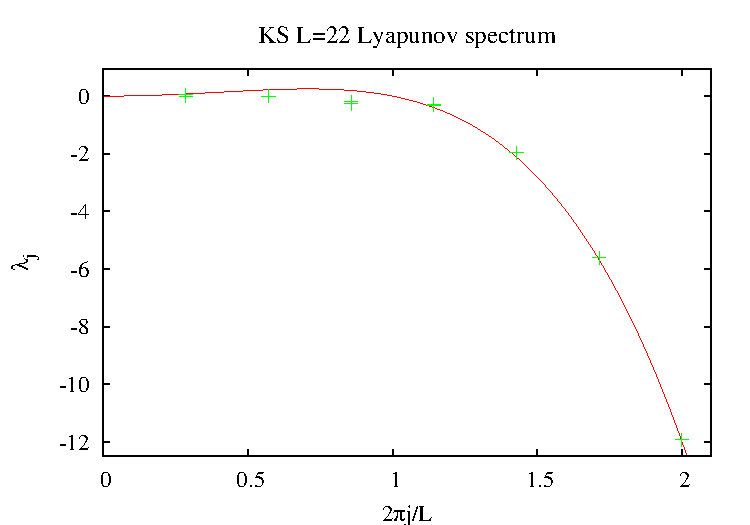
\includegraphics[width=0.40\textwidth]{lyapSpecRscld}
\caption{
(a)
Fig.~4 of
Yang \etal\rf{YaTaGiChRa08}:
Extensivity of the Lyapunov spectrum for the KS equation with
periodic b.c.. Inset: number of non-negative exponents (circles),
Kaplan-Yorke dimension (squares), metric entropy (diamonds,
multiplied by $50$), and number of physical Lyapunov vectors (triangles).
In perfect agreement with
\reffig{fig:lyapSpec}\,(b) here, plotted the same
(incorrect) way.
(b)
First 14 Lyapunov exponents $\lambda_j$ for the full
\statesp, periodic b.c. KS for $L=22$, from a 62 real Fourier
modes long-time simulation (from \refref{SCD07}).
The same as in part (a) and in \reffig{fig:lyapSpec}\,(b), but
abscissa is $j/\tildeL = 2 \pi j/L$, and each $j$ labels
the $\On{2}$ 2-dimensional irreducible representation
Lyapunov exponents pair.  Full line corresponds to
the stability eigenvalues
of the $u(x,t)=0$ stationary solution
$(j/\tildeL)^2- (j/\tildeL)^4$, for arbitrary system size $L$.
}
\label{fig:lyapSpecRscld}
\end{figure}


We also see
that the `physical' Lyapunov vectors are split into a less contracting 1/2
and more contracting 1/2 (different slopes in the
\reffig{fig:lyapSpecRscld}\,(a)). We
used to think the first 1/2 is the physically important one,
and say so in the arXiv version 2 of the article.
We stand corrected.

The Floquet eigenvectors of our (relative) periodic orbits are
what they call 'covariant,' so they should fit into their finite back/forth
time vectors like into a glove, whenever the respective state space
points are sufficiently close.

The main point of exploring the ergodic states space hierarchically
by periodic orbits is to tessellate it systematically, in the most
uniform way, by neighborhoods (linearized stable/unstable manifolds)
of periodic points. A periodic solution computed on a small system
size $L$, periodic b.c. is a solution on any multiple of $L$, and it comes
together with a smooth family of corresponding solutions for nearby
$L$'s.

I see prospects of a long and happy marriage here.

\item[2011-02-04 ES] Talked to Hugues Chat\'{e} and Kazumasa Takeuchi.
I was at CEA/Saclay for a thesis presentation today, bumped into Chat\'{e}
and
\HREF{http://daisy.phys.s.u-tokyo.ac.jp/student/kazumasa/}{Kazz}
(actually, it was more like invading their offices). Kazz updated me on
their latest work on Lyapunov vectors. We finally all agreed that we would give
the periodic orbit - Lyapunov vectors project a second try and arrange to meet
in Paris. I'll keep you posted.


\item[2011-02-07 ES] Sent Kazz an initial condition for a KS, $L=22$ \po\
\PO{10.25}.


\item[2011-02-09 Kazz] I tried your initial condition and it works perfectly!
I also tried to calculate the Lyapunov exponents associated to this {\po}.
The largest is about 0.03328, right? I'm not yet really sure about this value,
so it would be nice if you let me know the Lyapunov exponents you know for this {\po}.

\item[2011-02-11 ES] The Lyapunov exponent I have is 0.033163, so you
are pretty close. In fact this exponent has multiplicity two, and
there is no other positive exponent for this orbit.

\item[2011-02-11 Kazz] Great! All you are saying (multiplicity, only two positive
exponents) are exactly what I confirmed with that {\po}. I will soon have all
the necessary information regarding the physical/spurious Lyapunov vectors for that {\po}.

\item[2011-02-11 Kazz] Which quantities / properties do you have
analytically / numerically for these \po s in your methods? For instance,
if we know the time evolution operator for a {\po}, we can compute both
Lyapunov exponents and covariant Lyapunov vectors as eigenvalues and
eigenvectors of that operator. Do you have them? Or, the exponent values
you have are just computed by Bennetin's standard algorithm?

\renewcommand{\ssp}{x}

\item[2011-02-11 ES] We do not use Bennetin's method, but rather
something similar to what you just described. However, I am not sure how
you exactly define the time evolution operator, so I will describe with
details what we do (see \refrem{rem:Lyapunov} on \refpage{rem:Lyapunov} above).

Given an initial condition $\xInit$ and period $\period{p}$ of the prime
\po\ $p$, we integrate
the differential equations for the nonlinear flow
$d\ssp/dt=v(\ssp)$, and a differential equation for the \jacobianM\
from $t=0$ to $\period{p}$,:
\beq
    \deltaX(t) = \jMps^t(\xInit) \deltaX_0
    \,, \qquad
\jMps^t_{ij}(\xInit)
  =  \left. {\pde \ssp_i(t) \over \pde \ssp_j} \right|_{\ssp=\xInit}
\, .
\label{hOdes1}
\eeq
\beq
{d\over dt}\jMps^t(\xInit)
    = {\Mvar}(\ssp) \, \jMps^t(\xInit)
\,, \quad
\mbox{initial condition~~} \jMps^0(\xInit) = \matId
\,.
\ee{Bew_Miaw}
The {\stabmat} (\velgradmat)
\beq
{\Mvar}_{ij}(\ssp) ={\pde \vel_i(\ssp)\over \pde \ssp_j  }
\ee{DerMatrix1}
describes the instantaneous rate of shearing of the infinitesimal
neighborhood of $\ssp=\ssp(t)$
by the flow.
We write for its
eigen\-vectors $\jEigvec[j]$
(sometimes referred to as `covariant Lyapunov vectors,'
or, for \po s, as `Floquet vectors')
\beq
\jMps_{p}(\ssp)\, \jEigvec[j](\ssp)
   = \ExpaEig_{p,j} \,\jEigvec[j] (\ssp)
\,,\qquad
\ExpaEig_{p,j}
= \sign{p}^{(j)} e^{\eigExp[j]_p \period{p} }
\,.
\ee{cplxExpaEig}
where $\eigExp[j]_p = \eigRe[j]_p \pm i\eigIm[j]_p$
and $\sign{p}^{(j)}$ are independent of
$\ssp$.
The time-dependent
$\period{}$-periodic vector fields, such
as the flow linearized around a \po, are
described by Floquet theory. Hence
we refer to a \jacobianM\
evaluated on a periodic orbit either as
a {\em \FloquetM} or a {\em monodromy matrix}, to its
eigenvalues
$\ExpaEig_{p,j}$ as Floquet multipliers,
% \refeq{cplxExpaEig},
and to $\eigExp[j]_p = \eigRe[j]_p+i\eigIm[j]_p$ as Floquet or
characteristic exponents.



The eigenvalues $\ExpaEig_i$ of $\jMps^t(\xInit)$ are
the Floquet multipliers and its eigenvectors the Floquet eigenvectors
(the covariant Lyapunov vectors for \po s).

Then the $i$th `Lyapunov' exponent is the real part
$\eigRe[i] = \ln(|\ExpaEig_i|)/ T$ of the Floquet exponent..
Although we only have the eigenvalues in file, I could easily compute
the eigenvectors for comparison.

The problem with this approach is that, while we believe the leading
eigenvalues to be accurate, the highly contracting ones suffer from
numerical noise. So it would be hard for us to separate physical from
isolated eigenvectors based on this computation alone.


\item[2011-02-11 Kazz] Thank you for the explanation. That is exactly what
I meant by eigenvalues of the time evolution operator.

I compute the Lyapunov exponents (and the covariant vectors)
by Benettin's method (and by Ginelli's one). The only trick is that, each time
the trajectory $\ssp(t)$ returns to its original position $\ssp(0)$, \ie, at every cycle
of the orbit, I replace $\ssp(t)$ by its initial value $\ssp(0)$. This is to kill
numerical noise that would grow and eventually kick the trajectory
out of the periodic orbit. This method is accurate even for very small
exponent values.

\renewcommand{\ssp}{a}

\item[2011-03-10 Predrag] That's OK for the shortest orbits, but
for longer orbits it will have to be replaced by either section $\to$
section traversals (see multi-shooting in
\HREF{http://chaosbook.org/paper.shtml\#cycles}{ChaosBook.org}) or variational methods (see
\refref{CvitLanCrete02} and
\HREF{http://chaosbook.org/paper.shtml\#relax}{ChaosBook.org}).

\item[2011-02-18 Kazz]

\BFIG{1.0}   % width=#1\textwidth
{kaz-evolution}   % f_name.pdf
{}   % short caption text
{    % full caption text
\po\ \PO{10.25} [kaz-evolution]
}
{kaz-evolution}   % f-figure-label


Meantime I show you how my code integrates your {\po} (the first three in your
list), \reffig{kaz-evolution}. Indeed, I cannot integrate
it even during one period for the second one, which has a large
Floquet multiplier.

by the way, the period indicated in the file is actually half the real period?
The space-time plot indicates that...

\item[2011-02-18 ES]

Yes, this is the convention we follow in our paper\rf{SCD07}, sorry for not
bringing this to your attention. We define the period $T_p$ to be the
smallest time such that $u(x+T_p)=\gamma u(x,0)$, where $\gamma$ a
discrete symmetry transformation (here reflection $R$), see eq. (2.22) in
our paper and the discussion that follows it. All periodic orbits we
have found are thus pre-periodic, or \rpo s.
\PC{really all are \rpo s? I thought about 1/2 of this 40,000 -
60,000 were not?}
The evolution
$T_p$ to $2T_p$ is a repeat of the pre-periodic orbit which
is periodic in this case, as $R^2=1$ (and thus we can take the period to be $T_p$
rather than $2T_p$). You should take advantage of this
when computing Lyapunov exponents, integrating only from $0$ to $T_p$ and
then applying $R$ to $u(x,0)$ to get a new initial condition, before
integrating from $T_p$ to $2T_p$ and so on. I should have mentioned this
convention, but it is by now second nature to me.

By the way, what method do you use for integration? For the third
orbit, could you please compute $||u(x,2T_p)-u(x,0)||$ (or
$||u(x,T_p)-Ru(x,0)||$ where $R$ is reflection)? The choice of norm should
not be crucial. I ask because I think this is the best indicator of
reproducibility of the periodic orbits. For the second orbit, if you
could compute $||u(x,T_p)-Ru(x,0)||$, it might tell us that the
difference is not as large as the figure suggests.

\item[2011-02-21 Kazz]

\BFIG{1.0}   % width=#1\textwidth
{kaz-evolution2}   % f_name.pdf
{}   % short caption text
{    % full caption text
{\po} \PO{10.25} [kaz-evolution2]
}
{kaz-evolution2}   % f-figure-label


Thanks for the kind explanation. I should have read your
paper more carefully... I shall do this very soon.

Here I attach a figure, \reffig{kaz-evolution2}, showing
how a measure of the distance between a
trajectory and an orbit grows in time. The same trajectories and the orbits
as in the figure I send you last Friday are used. The dashed lines are the
growth rate expected from their Floquet multipliers and agree well with the
actual growth of the distance. Indeed, even for the second orbit the trajectory
stays close to it up to time $~2T_p$.

\item[2011-02-22 ES] In the last set of figures (evolution2.pdf), is $u(x,t)$
an orbit resulting from perturbing the initial condition of the periodic orbit?

\item[2011-02-23 Kazz] Concerning your question, the initial condition for u(x,t)
is exactly the one you sent to us. Just I integrated it and measured how
it deviates from the orbit because of the numerical noise.


\item[2011-02-20 Predrag] to Kazz:
I'm very glad that you and Evangelos are looking at the KS periodic solutions.
Attached is \refsect{sect:LyapKS} from out blog
(you probably have this already, but
I am not quite sure) - if you plot all cycle Floquet multipliers, can you try to
also plot them in the way suggested in my notes (it differs a bit from how you
had plotted them in Yang \etal\ paper\rf{YaTaGiChRa08})?
I was pleasantly surprised how well one
could see the physical/isolated boundary already for $L=22$.


\BFIG{1.0}   % width=#1\textwidth
{kaz2-PhysModes-cd}   % f_name.pdf
{}   % short caption text
{    % full caption text
Compare with frames (d) and (e) in \reffig{fig:lyapSpecCLG}.
{\po} \PO{10.25} [kaz2-PhysModes-cd]
}
{kaz2-PhysModes-cd}   % f-figure-label

\BFIG{1.0}   % width=#1\textwidth
{kaz4-VectCompar}   % f_name.pdf
{}   % short caption text
{    % full caption text
{\po} \PO{10.25} [kaz4-VectCompar]
}
{kaz4-VectCompar}   % f-figure-label

\BFIG{1.0}   % width=#1\textwidth
{kaz5-AngleTimeSeries}   % f_name.pdf
{}   % short caption text
{    % full caption text
{\po} \PO{10.25} [kaz5-AngleTimeSeries]
}
{kaz5-AngleTimeSeries}   % f-figure-label

\SFIG{kazUPOa}   % width=#1\textwidth
{}   % short caption text
{    % full caption text
{\po} \PO{10.25} [kazUPOa]
}
{kazUPOa}   % f-figure-label

\item[2011-02-21 Kazz]
I (with spirits of Hugues Chat\'e and Francesco Ginelli hovering above me)
have integrated some of
them and computed a number of quantities to elucidate the
physical/isolated separation of Lyapunov vectors. Here I show a
summary of preliminary results. I also have some questions to ask you
(see the end of the mail for them).


\textbf{Results}

Here we concentrate on (1) a ergodic trajectory generated from a random
initial condition, and (2) the first periodic orbit \PO{10.25},
$\period{p}=10.25336729174627$ in the list
Evangelos sent to me (called "{\po}a" in the attached
figures). The numerical integration of the {unstable \po} is done by replacing the
trajectory on each period by the initial condition of the {unstable \po}.
    \PC{to Evangelos - do we have a naming convention in \refref{SCD09b}
        and/or \refref{SiminosThesis} that we could follow here,
        instead of renaming every \po? {\bf ES:} No. We use
	$(T_p,\ell_p)=(.,.)$ to refer to a \rpo.}

% PC 2011-03-02: (b) generated by Kazz kaz2-PhysModes-b.png
\refFig{fig:lyapSpec1}\,(b)
and
% PC 2011-03-02: (b) generated by Kazz kaz2-PhysModes-a.png
\reffig{fig:lyapSpec}\,(b)
show the Lyapunov spectrum for
the trajectory and the {unstable \po}.

For the {unstable \po} the exponents are
given by the Floquet multipliers, as indeed confirmed quantitatively,
while for the ergodic trajectory they are different from but close to
those of the {unstable \po}, \refFig{fig:lyapSpec1}\,(b).
 %(top right figure).
Increasing the index, we
see the appearance of the step-wise structure (top left figure) like in
our Yang \etal\rf{YaTaGiChRa08} PRL.

\refFig{kaz2-PhysModes-cd} shows the hyperbolic isolation of the physical and
isolated Lyapunov vectors (similar to frames (d) and (e) in \reffig{fig:lyapSpecCLG}
from our PRL); they
CANNOT be defined solely from the Lyapunov exponents.). The quality of
the data is not satisfactory because of the present length of the
simulation, but we can see that there are at most 11 physical Lyapunov vectors.


\refFig{kaz4-VectCompar} compares the covariant Lyapunov vectors on the
ergodic trajectory with the Floquet vectors of the {unstable \po}. I monitored the
ergodic trajectory and used the instant when it gets closest to the {unstable \po}
during the simulation. The inset of the top left figure shows the
snapshot of the trajectory (blue) and the {unstable \po} (red) at that instant.

The other three subpanels compare the vector structure at the same
instant. Here the spatial shift between blue and red is already taken
into account, so that you can directly compare the two profiles. The
bottom two figures show the 6th and 9th Lyapunov vectors, which correspond to
real-valued Floquet multipliers of the {unstable \po} (thus Oseledec subspace is
not degenerated). We can see that the vectors of the ergodic trajectory
become quite close to the {unstable \po} counterparts (but not exactly; some are
better, others are not as good). For the Lyapunov vectors that correspond
to complex conjugate pairs of the Floquet multipliers, e.g. 1st and 2nd
ones, we have to compare a vector of the trajectory with arbitrary
linear combinations of the 1st and 2nd {unstable \po} vectors. Indeed, we can find
a combination that gives a structure similar to the vector of the
trajectory.

In short, as a ergodic trajectory wanders among {unstable \po}s, the vectors of the
trajectory change their shape incessantly to follow the vectors of the
closest {unstable \po} at each instant.


Now, the question is whether we can unambiguously define the physical
and isolated Lyapunov vectors for each periodic orbit, or not. We don't know how to
do this, because the angle between any Lyapunov vectors
of {unstable \po} varies periodically and thus does not reach 0 or
$\pi$ forever.

Moreover, we find that the hyperbolicity properties crucially depend on
the quality of the periodic orbit. See
\reffig{kaz5-AngleTimeSeries}, which shows
time-series of angles between given pairs of the Lyapunov vectors of the
{unstable \po}. Although the angle between Lyapunov vectors of index $\geq 11$ (correspond
to isolated Lyapunov vectors for the ergodic trajectory) stays close to $\pi/2$ with a
seemingly trivial time-evolution, the numerically computed angle is not
strictly $\pi/2$ and is subject to a very slow convergence (see the middle
panel). To test, I added a noise to the initial condition of the {unstable \po} and
computed the same quantities. While the angles for index $\leq 10$ do not
show significant changes, those for index $\geq 11$ show spurious
oscillations with long periods.

This is why we think that the quality of the periodic orbit is crucial.
It could be that, if we had an initial condition with infinite
precision, the angle for index $\geq 11$ are strictly orthogonal, and thus we
could define the isolated Lyapunov vectors from this strict orthogonality.


\textbf{Questions}

1) We wonder if we may define the physical and isolated Lyapunov vectors for
periodic orbits. Do you have any ideas, in particular from the viewpoint
of the Floquet multipliers and eigenvectors?

2) As shown above, the quality of the {unstable \po} initial conditions turns out
to be crucial. Do you have data with better resolutions? Or, is it
numerically difficult to compute {unstable \po}s with very high resolutions?

That's all for now. Any comments / questions are of course welcome!


\textbf{Kazz to Predrag} I made a plot of the Lyapunov spectrum of
the {unstable \po} (the same one as above) in the same way as you did. See \reffig{kaz{\po}a}
and {\po}a-lyap.dat (below). I hope this is the one you wanted.

                            \noindent
 3.3274529258200000e-2    \\
 3.3273022876699997e-2    \\
 1.2294744377000001e-5    \\
 -1.3236540275600000e-5    \\
 -7.2634814842399998e-5    \\
 -2.1629227416399999e-1    \\
 -2.6517234146000002e-1    \\
 -2.6516527982799998e-1    \\
 -3.3072168309500000e-1    \\
 -1.9602739059100001    \\
 -1.9673554279600001    \\
 -5.6025023421000002    \\
 -5.6042396292200003    \\
 -1.1925106699200001e+1    \\
 -1.1925523679299999e+1    \\
 -2.2011597078699999e+1    \\
 -2.2011657848500001e+1    \\
 -3.7116197744200001e+1    \\
 -3.7116202659300001e+1    \\
 -5.8760926784699997e+1    \\
 -5.8760926787599999e+1    \\
 -8.8935807811399997e+1    \\
 -8.8935807884699997e+1    \\

\item[2011-03-05 Predrag to Kazz] I do not understand your \po\ calculations.
For this short orbit I expect everything - all Floquet multipliers and
Floquet vectors to be good to a machine precision, or at least to - let's say -
$10^{-6}$?

\item[2011-03-05 Predrag]
I find
\reffig{fig:lyapSpec1}\,(b) amazing. The {\po} \PO{10.25} is
only exploring the $\infty$-dimensional \statesp\ as the
shortest 1-dimensional loop, while the ergodic trajectory is
wondering over the whole 11-dimensional (say Parisians) strange attractor
(inertial manifold) and still the entangled eigenvalues are so close.

\item[2011-03-07 Hugues]
That's because the {\po} \PO{10.25} is the least unstable of all
\po s.

\item[2011-03-07 Predrag] Easy to say, but in \refref{SCD07} we have
not noticed any concentration of the natural measure in the neighborhood of
this \po. That is perhaps because we have not quotiented
$\pS \to \pSRed = \pS/\SOn{2}$, and $\SOn{2}$ drifts can easily
mask a much simpler strange attractor\rf{SiCvi10,FrCv11}.


\item[2011-03-04 Evangelos]
I really can't follow this tessellation idea. My motivation to be
involved with this project at this point developed while reading Roweis
and Saul\rf{RoSa00}. I believe what we ought to do should be very close
to their way of thinking: construct linear local charts (bases) and then
bring them together to construct a global curvilinear embedding. In
contrast to their pattern recognition, empirical way to construct the
local charts, we can use information from the covariant Lyapunov vectors.

\item[2011-03-05 Predrag]
I agree in principle.

\item[2011-03-04 Evangelos]
I would prefer to work with \KS\ in the antisymmetric subspace, so that we do not
have to worry about the translational symmetry (remember that the periodic
orbits for $L=22$ are in the full space, rather that in the antisymmetric
subspace).

\item[2011-03-07 Hugues]
I agree, shifts are killing us.

\item[2011-03-05 Predrag]
I agree.
    \PCedit{
[revised 2011-03-10: I disagree, see comment below]
    }


\item[2011-03-04 Evangelos]
The local charts can be provided by the physical covariant Lyapunov
vectors computed on a set of the most important \po s. Then we only need
to implement the final step in the procedure of Roweis and
Saul\rf{RoSa00}, which involves solving a minimization problem for the
global coordinates and should be computationally tractable if a truly
low-dimensional embedding exists.

\item[2011-03-05 Predrag]
We cannot tessellate with \po s; we can only work with \emph{periodic
points}, hence we need to understand what Floquet vectors (AKA `covariant
Lyapunov' vectors evaluated on \po s) tell us about the `physical
dimension' of the local \Poincare section.

\item[2011-03-04 Evangelos]
How could a trajectory be confined to a \Poincare section? You seem
to talk about local charts in \refsect{sec:chart}, rather than \Poincare sections.

\item[2011-03-05 Predrag]
Ant is not following a \emph{trajectory}, ant is moving \emph{transversely}
to the time flow, for example: if the continuous time trajectory has one
unstable eigen-direction, it sweeps out a 2-dimensional unstable manifold,
whose \Poincare section is 1-dimensional curve that the ant could follow.

\item[2011-03-04 Evangelos]
If we manage to use local \Poincare sections to reduce the flow to a
discrete map (or maps) before applying this procedure, we would then only
need one (or a few) representative point(s) per periodic orbit for our
local charts, rather than points along the full orbit. However, we know
this is tricky to do in a high-dimensional space, before an embedding is
available.

\item[2011-03-05 Predrag]
\HREF{http://en.wikipedia.org/wiki/String_Quartet_No._16_(Beethoven)}
{Es muss sein!} No sense can be made out of a collection of \po s unless
they and their Floquet vectors are reduced onto  \Poincare sections.

\item[2011-03-04 Evangelos]
In any case, while I can see many local \Poincare sections working
together, either before or after the global coordinates are found, I
cannot see how a tessellation as you describe it here would work.
\Poincare sections are designed to pierce the flow (so the ant we follow
would leave the section immediately) and good sections should be
transverse, not tangent to the attractor.

\item[2011-03-05 Predrag] Grave misunderstanding. The continuous group
that is being reduced by \Poincare sections is the evolution in time.
After the reduction of continuous time to discrete time, what remains are
the affine hyperplanes (local \Poincare sections) which are
\emph{tangent} to the strange attractor; the ant is not crawling in the
time direction, she is crawling (for example) along the unstable manifold
heteroclinic section as it is seen within the \Poincare sections, not the
time trajectory traced out in the full \statesp.

\item[2011-03-02 Evangelos] First meeting's wisdom:
\begin{itemize}
 \item[2011-03-02 Parisians] We
 \HREF{http://en.wikisource.org/wiki/Gargantua/Chapter_XVI}{Parisians}
  all agree that it's best to work on antisymmetric subspace KS.

\item[2011-03-10 Predrag]
    \PCedit{
I'm very worried about this development. We have settled in
\refref{lanCvit07} on $L=22$ as the smallest system size for which the
translationally invariant KS is empirically `shmurbulent.' We cannot work
with \KS\ in the antisymmetric subspace at $L=22$, because there is no
chaos there - that's why Lan and I worked\rf{lanCvit07} at  $L = 38.5$.
We cannot work with \KS\ with the fixed $u(0)=u(L)=0$ boundary conditions
at $L=22$, because there will be no shmurbulence there either - when the
ends are pinned down, one needs a larger cell to approach the onset of
shmurbulence, that's why the antisymmetric subspace required going up to
$L = 38.5$. Besides, for small $L$ the boundary effects will dominate the
dynamics, the \statesp\ geometry will be very different, and what we
learn there will not scale to larger $L$. What was so elegant about
analysis\rf{SCD07} of  $L=22$ system is that the geometry of the
\statesp\ was so much more beautiful than what it is for the $L = 38.5$
antisymmetric subspace. Since then we have lost fear of continuous
symmetries\rf{SiCvi10,FrCv11}. And continuous symmetries are the
physically interesting case. In summary, going to fixed b.c. is ugly,
unphysical, and to add insult to injury, it would necessitate a whole new
fishing expedition, abandoning all the wisdom we already have in the
$L=22$ case.
    } %end \PCedit{


\end{itemize}



\item[2011-03-02 Evangelos] First meeting's numerics:
\begin{itemize}
 \item Evangelos will do the shooting for periodic orbits
	(we need to decide on system size). He hopes he will find the time \ldots
 \item Kazz uses an implicit second order Adams(-Moulton) method (see post of
	2011-03-09), with pseudospectral space discretization.
	He uses some prescription for anti-aliasing, in order to keep the large wavenumbers
	and corresponding isolated Lyapunov vectors uncontaminated. Uses numerical
	recipes for FFT. (ES suggests switching to FFTW as numerical recipes FFT is
	known to be unreliable in double precision.)
 \item Evangelos uses explicit fourth order Runge-Kutta with exponential
	time differencing (see \refref{ks05com}) and pseudospectral space
	discretization. He uses brute force anti-aliasing (increases resolution
	to the point that only Lyapunov vectors already at round-off are affected by
	aliasing). He uses FFTW.
    \PC{can you identify this pesky reference 'ks05com'?}
 \item We agreed that a good strategy would be that Kazz implements a simple
	Newton routine, so that he can refine the orbits I give him. I've
	pointed him to Chaosbook chapters, my own first year report on Newton's
	method for periodic orbits and my thesis.
 \item I've also agreed to give Kazz the backbone of my integrator routines
	(and also pointed him to \refref{ks05com}). Kazz is suspicious towards
	Trefethen's algorithm, he thinks that the integrating factor trick might
	lead to under-resolved large wavenumbers and problematic isolated
	Lyapunov vectors (and that the implicit method performs better in this
	respect). I can't argue in favor of one or the other integrator.
 \item I am also thinking to try to implement anti-aliasing and see
	if agreement improves.
\end{itemize}

\item[2011-03-09 Kazz] to Evangelos:
Before your mail I made a code to improve the quality of the periodic orbits
and it works very well. Now, with my integrator, the norm of distance
(with square root) after one cycle is on the order of $10^{-13}$ for the orbit
I focus on, and the trajectory stays nearby over $40$ periods, to be compared
with $10$ for the original orbit data. I restarted all the calculations
with this improved orbit.

To answer your question, my code uses the splitting method with the
2nd-order implicit method
\HREF{http://en.wikipedia.org/wiki/Linear_multistep_method}{(Adams-Moulton)}
for the linear terms and the 2nd-order Runge-Kutta
\HREF{http://en.wikipedia.org/wiki/Heun\%27s_method}{(Heun method)}
for the nonlinear term.

For the aliasing, I use at least $(3N+1)$ spatial points when computing
the nonlinear term, where $N$ is the wavenumber cutoff of the Fourier modes.
Under this condition the pseudospectral method is exact
(equivalent with the spectral method apart from the computational cost).

\BFIG{1.0}   % width=#1\textwidth
{kaz-fig-temp}   % f_name.pdf
{}   % short caption text
{    % full caption text
{\po} \PO{10.25} [kaz-fig-temp]
}
{kaz-fig-temp}   % f-figure-label

\item[2011-03-10 Kazz] To refine the orbits I use Newton's method,
but I adapted it to apply to half a period, playing with the reflection
symmetry. That is to say, instead of considering
\[
  (I-J(u))(u'-u) - vt = -(u-f(u))\,
\]
I use
\beq
  (R-J(u))(u'-u) - vt = -(Ru-f(u))\,
\ee{eq:preper-newt} where $R$ is the operator
for the reflection, i.e., $Ru(x) = -u(-x)$.
It is better, not only because the integration time is half, but also because
the reference coordinate $x_0$ for the reflection $u(x,t)=-u(x_0-x,t+T_p)$
is automatically set to be 0.

That said, I looked at the results from the refined orbit, and found
that the results do not change. The angle between spurious Lyapunov vectors oscillates
always with a finite amplitude.

\item[2011-03-10 ES] My bad here, I forgot to mention to Kazz that we
use \refeq{eq:preper-newt} for pre-periodic orbits \ldots

\item[2011-03-10 Ruslan] {\em Comment on the numerical approximation of the KS flow}\\
I would suggest not to worry too much about the accuracy of the numerical
approximation of the KS flow.  Instead, it is better, in my opinion, to
adopt the viewpoint that one investigates the properties not of the KS
flow, but of the map defined by the numerical integrator of the \KSe,
which approximates the solutions of the \KSe.  As long as the orbits of
the map resemble the solutions of the flow (think of it in terms of
shadowing), the results of our investigation of the map will faithfully
represent those for the KS flow.  So, it doesn't matter whether one
investigates the Kassam-Trefethen map or the Adam-Moulton-RK map: the
qualitative picture will be the same.

The neat thing about Kassam-Trefethen map is that it solves the linear
part of the KS flow exactly, thus eliminating the problem of the
stiffness of the linear part, and thus allowing to use a much larger time
step.  Implicit Adams-Moulton also deals with the stiffness, but it
solves the linear part only approximately, so it is likely to be less
accurate if used with the same time step.

From the same viewpoint, there is also no need, in my opinion, to use
anti-aliasing.  If a better approximation of the KS flow is needed, just
include more modes into the map and decrease the time step.  Of course,
if Kazz already implemented anti-aliasing, then there is no harm in using
it, provided it doesn't increase the flops count too much.

\item[2011-02-21 Kazz]
If the isolated Lyapunov vectors of
{unstable \po}s are strictly orthogonal, it means that the \jacobianM\ for a
cycle can be decomposed to two parts, one of which would be an
orthogonal submatrix. Does that seem likely to you?

\item[2011-03-10 Ruslan]
I don't see why we should expect higher Lyapunov vectors to be {\em
exactly} orthogonal.  Since all Lyapunov vectors in the \KSe\ are coupled
though the nonlinear term, the deviation from orthogonality should be
proportional to the strength of this coupling.  Of course this coupling
is very weak for higher Lyapunov vectors and decreases exponentially with
increasing mode number.  But if we measure with sufficient resolution,
which is what Kazz does, we'll observe the deviation from orthogonality
for any higher mode, whether anti-aliased or not.  Or am I wrong?

\item[2011-03-10 Predrag] My belief too. There is no reason to require
non-physical Floquet vectors to be pure, orthogonal Fourier modes: all we
need is that perturbations along these directions are pushed back into
the attractor without being entangled along it...

\item[2011-03-11 Ruslan] It seems to me that the behavior of the isolated
Lyapunov vectors in the \KSe\ is rather easy to understand.  Since they
are essentially generated by the linear part of the \KSe, they will be
nothing else but the Fourier modes living in mutually orthogonal planes.
That is, they are the eigenvectors of the \jacobianM\ of the trivial
equilibrium $u = 0$, just slightly perturbed by the nonlinear coupling.
But since, as I already said, this perturbation decays exponentially with
the mode number, it is negligible for high enough modes.  So, to answer
Kazz's question, the strongly contracting eigenvectors of the \jacobianM\
of a cycle should be essentially orthogonal to one another as well as to
the subspace spanned by the expanding and weakly contracting eigenvectors
(i.e. the subspace where the physical Lyapunov vectors live).

\item[2011-06-28 Evangelos]
Met with Kazz at \HREF{http://cct11.cpt.univ-mrs.fr/}{CCT11 conference}
at Marseilles and discussed about their progress with Lyapunov vectors
for periodic orbits. To my understanding, the main points are: Kazz
\etal, identify generic orbits that come close to a periodic orbit. They
use the vector defined by the points of minimal distance along these two
trajectories as a local approximation to the ``inertial manifold.''
However, some of the Lyapunov vectors computed along the periodic orbit
and the generic trajectory are not identical or even similar (at the
points of minimal distance). Kazz argues that it is not possible to
define physical and isolated modes for periodic orbits (in his numerics
the number of physical dimensions inferred from a periodic orbit would
be, in general, different from the number of physical dimensions inferred
from a generic orbit).

\item[2011-06-28 Predrag] I will deal with this in bits:
First, not being in frequent contact is not working for me - I
do not know what is being computed or why. Are we in the \KS\
antisymmetric subspace at\rf{lanCvit07} $L = 38.5$, or the
full space at $L=22$? As I wrote above in the {\bf 2011-03-10}
entry, I believe we cannot work in the \KS\ antisymmetric
subspace at $L=22$, as there is no shmurbulence there. If Kazz
is integrating trajectories in the full space at $L=22$, he
\emph{must} quotient the translational $\SOn{2}$, otherwise
there is no way to define the (locally minimal) Euclidean
distance(s) between a \po\ and a generic long-time trajectory\rf{FrCv11}.

\item[2011-07-22 Evangelos] Spatial shift in eq. (2) of 2011-07-21 draft seems
to take care of that, although this approach seems to be somewhat inefficient.
A question: Is the spatial shift a multiple of the spatial discretization step?
If yes, then this means that you probably overestimate the distance of minimum
approach based on eq. (2). You should then refine the comparison by introducing
a local slice as in \refrefs{SiCvi10,FrCv11}.


\item[2011-06-28 Predrag]
Using ``the vector defined by the points of minimal distance along these two
trajectories as a local approximation to the inertial manifold'' makes no sense to me.
The local approximation to the inertial manifold is spanned by the transverse
\po\ Floquet eigenvectors at that periodic point (simplest to take a local \Poincare section
normal to $\vel(\ssp)$ at $\ssp$).

\item[2011-06-28 Predrag]
If the generic trajectory is close the periodic point in a direction
along its unstable manifold, it is close. If it belongs to a different fold of the
unstable manifold, than it is far away and can have quite different local
tangent space.

If the two points are close, the periodic point tangent space
eigen-directions should be close to the covariant vectors at the nearby generic
point, as they are probing the same stable / unstable manifolds structure in the
linear neighborhood that includes them both.

\item[2011-07-22 Evangelos]
I've actually raised the objection about the generic trajectory belonging to a
different fold of the unstable manifold of the periodic orbit to Kazz in our
discussion at Marseilles. His
counter-argument is, I think, based on figure 5(c) of 2011-07-21 draft. His
claim is that since the angle tends to zero as the generic trajectory approaches
the periodic orbit the approach has to be along the unstable manifold.
However, I am not convinced that we can numerically tell the difference
if the minimum distance along the local unstable
eigen-direction is much larger than the separation of folds of the unstable
manifold. Kazz, could you please clarify and give as more insight?

\item[2011-06-26 Kazz] It is not possible to
define physical and isolated modes for periodic orbits (in my numerics
the number of physical dimensions inferred from a periodic orbit would
be, in general, different from the number of physical dimensions inferred
from a generic orbit)

\item[2011-06-28 Predrag]
A short \po\ might be quite hyperbolic, \ie\ never get close to any
tangencies (small angles between leading Floquet eigenvectors). The longer ones
should probe heteroclinic tangencies a bit better...

\item[2011-08-09 Predrag] For comments to Takeuchi and Chat\'e\rf{TaCh11}
\emph{Can the inertial manifold be captured by unstable periodic
orbits?}, see {\bf [2011-07-21]} entry, \refsect{sec:TaCh11}.

\item[2011-08-17 Evangelos]
I've just arrived to Dresden and found out that Hugues will
spend a year in the Institute heading a study group and Kazz will come
here for a workshop. So I'll get a chance to talk discuss with them.

\item[2011-08-17 Evangelos]
Kazz works in full space but studies
periodic orbits. You and me know that relative periodic orbits are the
relevant objects that are expected to capture the dynamics in presence
of translational symmetry, so why not try them instead?

\item[2011-08-17 Predrag]
Here is my proposal to you and Ruslan. You have some 40,000 \rpo s. Why
not take a point on the Kazz favorite cycle
\PO{10.25} as the template $\slicep$, and pick from
the 40,000 \rpo s the set of the closest ones to it in its slice. As they
are cycles in {\pSRed} you need to also make a local Poincar\'e section
through template point $\slicep$ (within the slice), normal to the
velocity vector $\velRed(\slicep)$, to find the closest passage. Some are
probably as close as the Kazz ergodic trajectory closest passage. For
each of the close ones you have the 9-12 leading eigenvectors, their
orientations information on where you are on stable/unstable manifolds,
and their relative separation vectors. Those Kazz will need to check,
show they are in the `physical' 9 dimensions.

\item[2011-08-25 Hugues, Predrag]
Evangelos is here sitting with me, and we tried to figure out what you
meant exactly. We have a proposal for something (hopefully) close to your
idea:
\begin{enumerate}
  \item Take Kazz `favorite orbit' \PO{10.25} (or a few of them). For
  this one, we know the vectors pretty well, all along the cycle.
    {\bf [2011-08-25 Predrag]} Pick a \emph{specific point}
    $\ssp_{\PO{10.25}}$ on the Kazz favorite cycle \PO{10.25} as the
    \template\ $\slicep = \ssp_{\PO{10.25}}$. As you will use $\slicep$
    to fix both the slice and the Poincar\'e section, some choices might
    be better than others: I am not sure how to pick this starting point.
    The local Poincar\'e section through template point $\slicep$ (within
    the slice) is picked normal to the velocity vector
    $\velRed(\slicep)$. The Floquet vectors are computed \emph{within}
    both the slice and the Poincar\'e section; the computation is
    described in the ChaosBook Section 5.3
    \HREF{http://chaosbook.org/chapters/invariants.pdf} {Stability of
    Poincar\'e map cycles}.


  \item Take the 40000 or so \po s available; for each near one,
  determine the closest point to the \template\ point \PO{10.25} (by
  "slicing" or more pedestrian methods).
      {\bf [2011-08-25 Predrag]} Slicing + Poincar\'e is, \emph{by
      definition}, the closest distance between the \emph{\template\
      point} $\ssp_{\PO{10.25}}$ and the \po\ (or \rpo) $p$. There are
      \emph{no} more pedestrian methods that work. If they exist, please
      enlighten me; what Kazz does is unecessarily laborious and
      inaccurate. Nothing can be said about the topology of inertial
      manifold unless symmetry reduction is implemented first. We have
      implemented slicing on 3D Navier-Stokes full resolution pipe flow
      ($10^5$ dimensions), so what do you fear about slicing $10^2$
      dimensions but the fear itself?


  \item At this closest point $\ssp_p$ on {\po} $p$, we have a minimal
  distance $\|u_p\|$ to the \emph{\template\ point} $\ssp_{\PO{10.25}}$,
  and the corresponding difference vector $u_p$. We can then compute the
  angle between vector $u$ and the subspace spanned by the $n$~first
  Floquet vectors of the \template\ point  \PO{10.25} (at the point of
  closest distance of course).

  \item Plot this angle (or its mean), as a function of $\|u\|$ for the
  nearest 10-100 out of the 40000 (relative) \po s. This could give the
  same result as our Fig.5c: if you take fewer vectors than the
  "physical" number, then the angle is bounded away from zero, but if you
  take the "right" number (or more), then the angle goes linearly to zero
  with $\|u\|$. Throw away `near' \po s which are near in Euclidean
  metric, but are isolated and off the local tangent space to the
  unstable (or `physical') manifold.

  \item This set of periodic \emph{points} covers a linearized tile
  around the \template\ point \PO{10.25}. Now take one of them toward the
  edge of the tile as the new \template\ point, and repeat. If that one
  has a small physical dimension for a finite neighborhood, we have a
  chance of tiling the entire inertial manifold as in
  \reffig{fig:Tesselate}.
\end{enumerate}
If, indeed, similar behavior is observed from just looking at \po s, then
the dimension of the ``physical manifold'' has been indeed calculated
using strictly only \po s.....  ah ah!

\item[2011-08-17 Evangelos]
By the way, do you understand how Kazz handles spatial shifts? After a
long exchange of emails it seems that I don't.

\item[2011-08-17 Predrag]
I believe he does it what was the standard way before the invention of
slicing. Following ChaosBook:

{\SOn{2} irreducible representations:}
Expand a smooth periodic function $u(\gSpace + 2\pi) =
u(\gSpace)$ as a Fourier series
\beq
u(\gSpace) = a_0 + \sum_{m=1}^\infty \left(
a_m \cos m \gSpace + b_m \sin m \gSpace
                               \right)
\,.
\ee{FourierExp}
The matrix representation of the \SOn{2}\ action
on the $m$th Fourier coefficient pair
$(a_m,b_m)$ is
\beq
\LieEl^{(m)}(\gSpace') \,=\,  \left(\barr{cc}
 ~\cos m \gSpace'  & \sin m \gSpace' \\
 -\sin m \gSpace'  & \cos m \gSpace'
    \earr\right)
\,,
\ee{SO2irrepAlg-m}
For each ergodic trajectory point he runs $\theta$ in some interval and
finds the minimal distance to the periodic point (their paper says that).
Though I am not sure that this is what he really does.

Sorry, getting too late - need to go to bed.

\item[2011-09-12 Evangelos] Talked with Kazz, Hugues and Francesco (2011-09-12).
The main points are:
\begin{itemize}
 \item No one wants to discuss slice fixing details, so I did not insist.
 \item I explained [2011-06-28 Predrag] comment on the discrepancy of some of the
	Lyapunov vectors as computed on a chaotic trajectory and a periodic
	orbit in Fig 3 of \rf{TaCh11}. Francesco says a math paper shows
	continuity of Lyapunov vectors but he will check the assumptions
	(and will send me the reference).
 \item We agreed to follow Predrag's suggestion and check the
	role of non-hyper\-bolic periodic orbits. Kazz will try to identify
	regions in state space where hyper\-bolicity seems to
	be violated and will give me some guesses for periodic orbits.
\end{itemize}

\item[2011-09-12 Predrag] This aversion to slicing is a pain. None of the
problems with continuous symmetries can be done without it, but so far I
have only gotten Willis converted\rf{ACHKW11}
\HREF{http://www.cns.gatech.edu/~predrag/papers/ACHKW11.pdf}
{(a rough draft is here)}, and that is because in pipes the streamwise
continuous symmetry is $\SOn{2}$ (no discrete reflections) so
\emph{nothing} can be done without slicing. Not slicing in KS, CLGe, and
\pCf\ is simply wrong - one cannot organize the \statesp\ without it. My
impression from the {\bf [2011-07-27 Kazz 2 Evangelos]} comments in
\refsect{sec:TaCh11} is that Kazz is confused about what slicing
is, but believes he understands it. Can you get EVO running in an MPI-KS
conference room? Maybe I can get them to listen, through a webinar on
slicing.

\item[2011-09-12 Predrag] It probably suffices that Kazz identifies 	
regions in state space where hyper\-bolicity seems to 	be violated. Once
you have it, you can get a guess from a long time recurrence plot for the
nearest periodic orbits.

\item[2011-09-12 Predrag] I do not like that in their way of thinking,
physical dimension is a consequence of non-hyperbolicity. Strange
attractors are not structurally stable, and minute changes in dynamics
totally change long-time non-hyperbolicities - infinitely many long \po s
are born and destroyed for every system parameter change; does that mean
that physical dimension changes? I guess it does, because if a stable
orbit is created, their physical dimension goes to zero or one within
that basin of attraction...

\item[2011-09-12 Evangelos 2 Predrag] Here non-hyperbolic periodic orbit follows
the convention of ChaosBook.org, right? It seems that Kazz and Hugues follow a
different convention. I will have to talk with Hugues.

\item[2011-09-12 Predrag]                           \toCB
A precise definition would be a \po\ or \rpo\ with an exact (dynamical,
not symmetry induced) marginal eigenvalue, $\eigExp[j] = 0$, as in
ChaosBook Chapter ``Intermittency''. But in this context we are looking
for (relative, I hope the light will go on for Kazz at some point) \po s
with one or several positive Floquet exponents whose value is much below
the Lyapunov exponents values. I expect it could be any of the 'physical'
eigen-directions exponents, meaning that different directions get
entangled pairwise, at different regions of the \statesp.

\item[2011-08-25 Predrag]
Until we do some Poincar\'e sections and have a symbolic dynamics
labeling, let's call \PO{10.25} the \po\ with
$\period{p}=10.25336729174627$, by specifying the period to 4 significant
digits, and \RPO{16.3?} for \rpo\ with
$(\period{p},\shift_p)=(16.3,2.86)$ - here I do not have the numbers
handy, sorry. In principle we need both the period and the shift
$(\period{p},\shift_p)=(.,.)$ to refer to a \rpo, but let's hope for
purposes at hand time is enough to distinguish any two \rpo s explicitly
cited.

%%%%%%%%%%%%%%%%%%%%%%%%%%%%%%%%%%%%%%%%%%%%%%%%%%%%%%%
\begin{figure}
 % ES: Generated by siminos/chao/matlab/ruslan/ks22ppo_angl.m
 % and siminos/chao/matlab/ruslan/ks22ppo_angl_plot.m
 (a)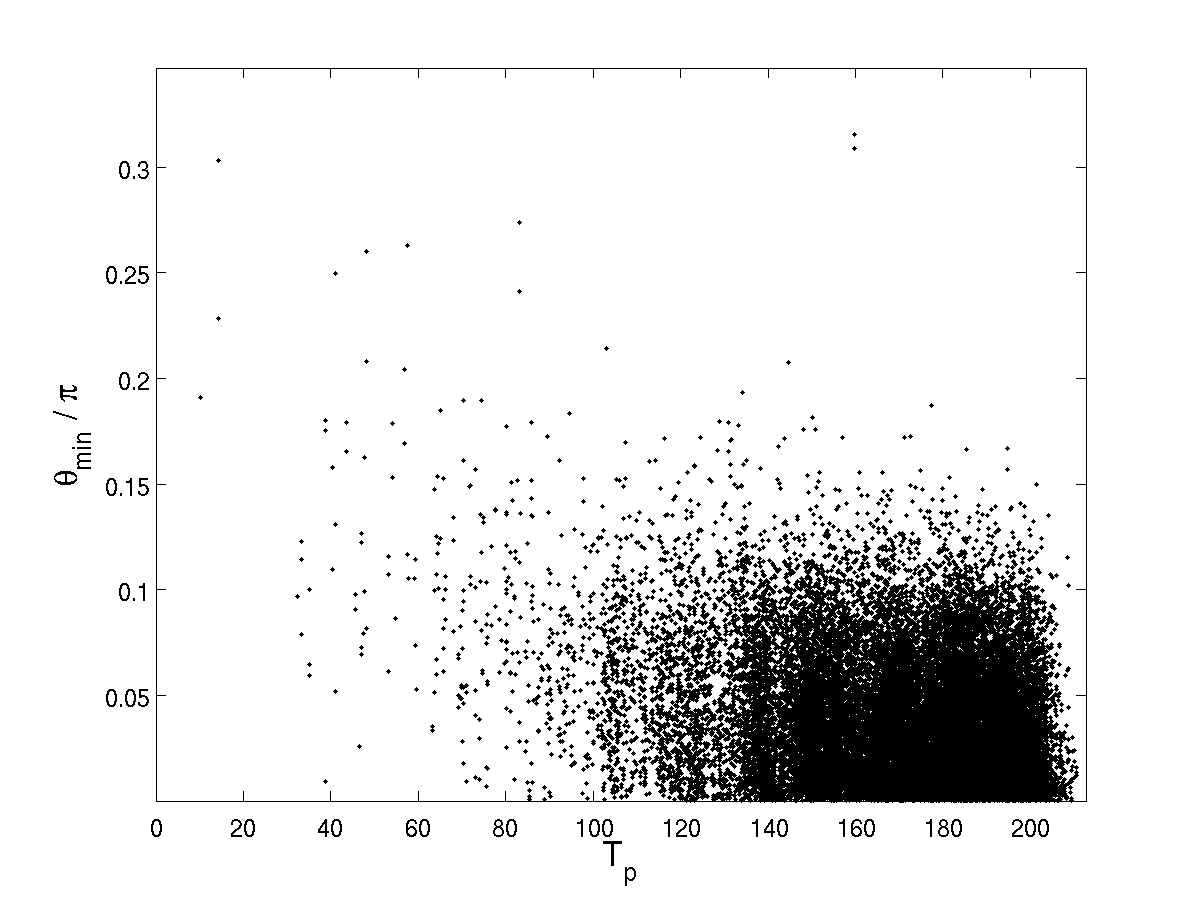
\includegraphics[width=0.44\textwidth]{ks22ppo_min_angle}
 ~(b)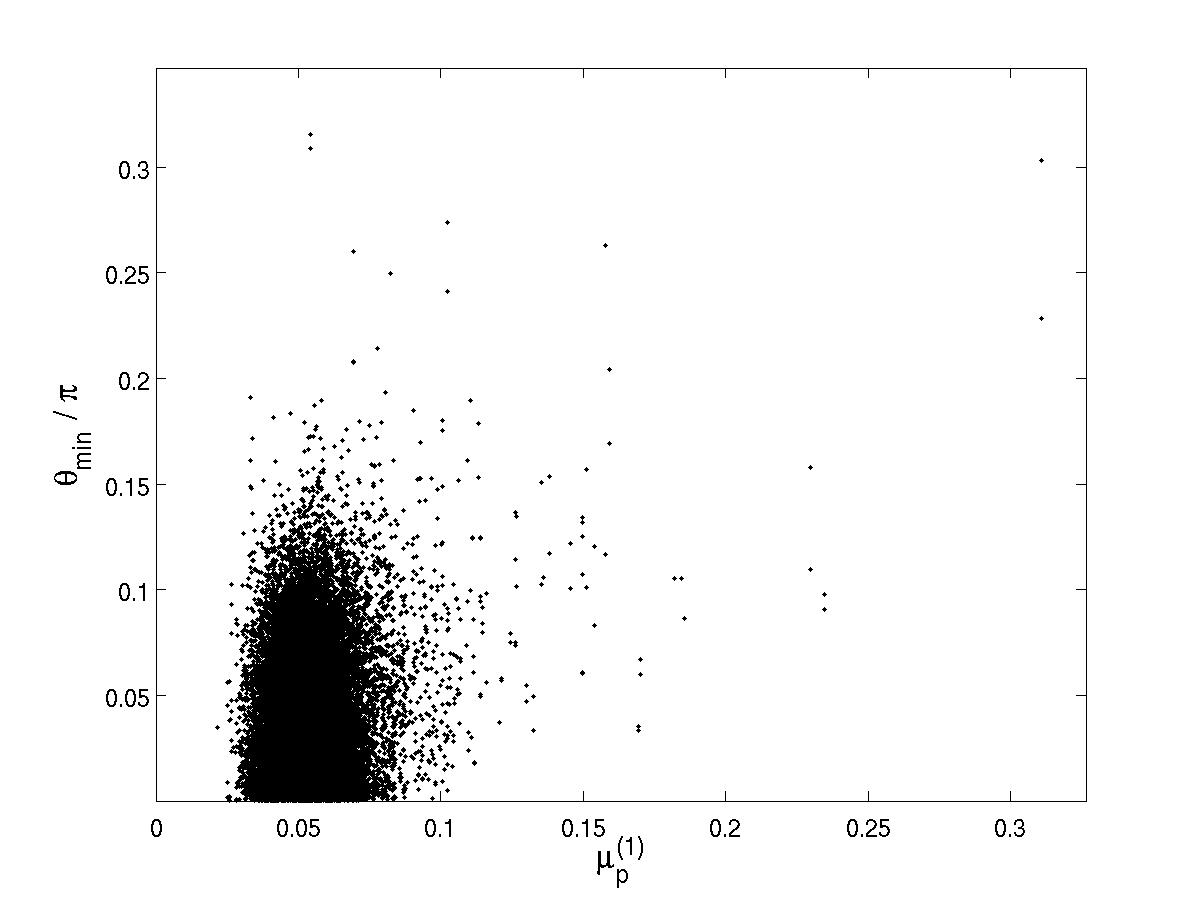
\includegraphics[width=0.44\textwidth]{ks22ppo_min_angle_floq}\\
 (c)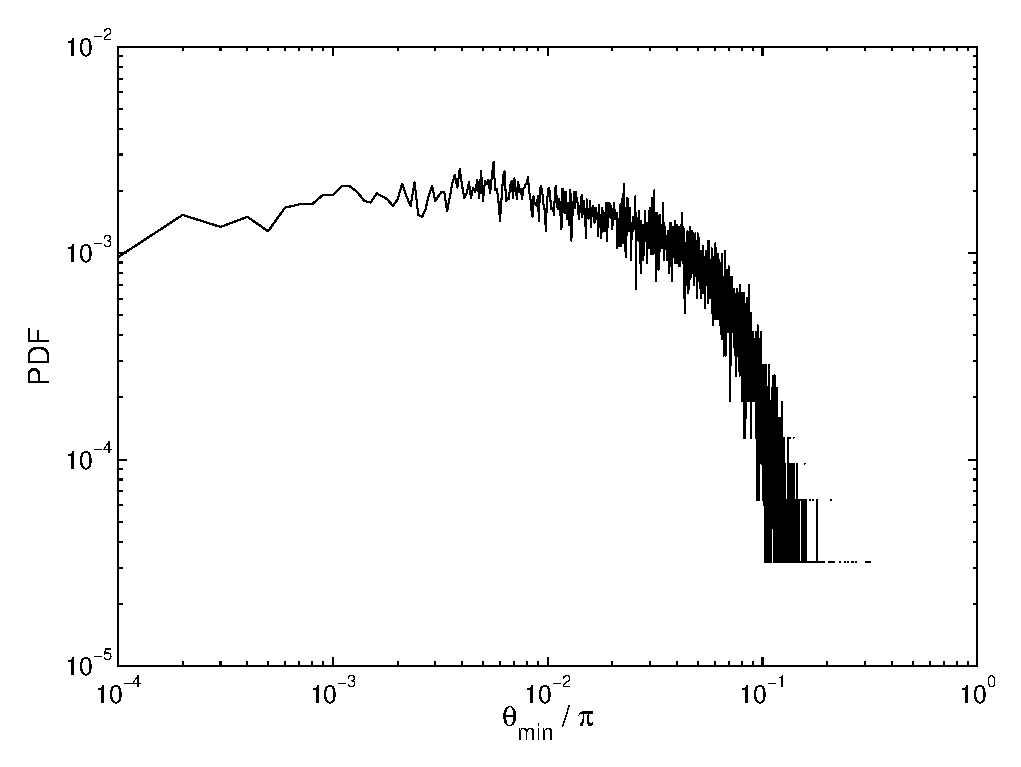
\includegraphics[width=0.47\textwidth]{ks22ppo_min_angle_pdf}
\caption{
Approximate minimum angle of pairs of Floquet eigenvectors
$\jEigvec[i],\, \jEigvec[j]$, $i,j=1,\ldots 5,\, i\neq j$ (angle was not
computed for marginal directions) along numerically computed points of
periodic orbits, (a) versus the period of the orbit $T_p$. Red solid line
shows the average minimum angle over bins of $\Delta T_p=15$. (b)
Minimum angle versus the largest Floquet exponent $\eigRe[1]_p$.
(c) Probability density function of the minimum angles shown in panel
(a). KS system size $L=22$, 16 Fourier modes truncation.
}
\label{fig:ks22ppo_min_angle}
\end{figure}
%%%%%%%%%%%%%%%%%%%%%%%%%%%%%%%%%%%%%%%%%%%%%%%%%%%%%%%


\item[2011-10-26 Evangelos]
I've looked at the minimum angles of pairs of leading Floquet vectors
across all periodic orbits (not relative periodic) in Ruslan's data. I
could reliably get the first five Floquet vectors for about $10,000$
orbits with periods $T\in[10.25, 210.61]$ out of approximately $30,000$
orbits in the set. Results are shown in \reffig{fig:ks22ppo_min_angle}.
Largest (minimum) angle detected was $0.3155\pi$, smallest one was
$3\times10^{-7}\pi$.

\item[2011-10-26 Predrag] \refFig{fig:ks22ppo_min_angle} is really
interesting. Plotting the angle {\em vs} the leading Floquet exponent $\eigRe[1]_p$
rather than time \period{p} is probably more informative.


The \po s are not really \po s (there are none in the
antisymmetric subspace for $L=22$, right?), but these pre-periodic
things that drift in the group tangent direction and then return? [{\bf ES}: yes]
You are using right (expanding forward in time) Floquet eigenvectors
$\jEigvec[i]$? [{\bf ES}: yes] Maybe for contracting directions one has to switch to the
left Floquet eigenvectors $\jEigvecT[i]$. Hugues will know.
[{\bf ES 2011-10-27}: Just to be clear about what I do compute: I use the Jacobian
calculated over a complete period ($2T_p$) to compute Floquet eigenvectors.
Any objection? {\bf PC 2011-10-27}: dunno...]

You are right to ignore the marginal directions, but it might be that
when you do it correctly (\Poincare\ in time direction, \slice\ in \SOn{2}
direction) you will get much larger angles, as $\jEigvec[i]$ might form
very non-normal narrow pencils of eigenvectors, stretched out along the
flow direction.

I only have H\'enon intuition, not sure how it will play out for higher
dimensions. If my hunch is right, I think for starters you should select
only the \po s for which the leading pair $\jEigvec[1] \cdot \jEigvec[2]$
has a small smallest angle, and then plot the point on the cycle where
the angle is smallest, projected on $3D$ a physical coordinate
frame\rf{GHCW07,SCD07} (no Fourier mode projections, please). It really
should be plotted in a \Poincare\ in time direction, \slice in \SOn{2}
direction, but we have not gotten that far. Note also that this $\cdot$
product has no invariant meaning, the eigenframe is not orthogonal.

If we are lucky these points
will align, telling us where the primary folds (in the sense of H\'enon
pruning front theory, \refchap{c-Henon}). But probably that will happen
only in a Poincar\'e section, in the full flow the folds in unstable
manifold have an extra, longitudinal dimension, which makes them a hell
to visualize. Ditto the \SOn{2} tangent AKA drift direction.

Once we see where these folds are in the \statesp\ we'll think of less
painful ways of nailing them down then by the close \po\ passages.

Small angles in $\jEigvec[2] \cdot \jEigvec[3]$, \etc, have to do with
`non-leading' folds in the less expanding unstable manifold directions,
so they will be trickier to visualize. Guys who generalize baker maps to
volumes call that 'hyperchaos'. I have not been able to visualize these
higher-dimensional folds. Again, just my pruning front hunch, might play
out differently when there are 8 physical dimensions.

\item[2011-10-26 Predrag] Note that the leading Lyapunov exponent is
$\Lyap = 0.048$ (see {\bf [2009-09-13 Ruslan]} above), and all
$\eigRe[1]_p \geq 0.024$ in \reffig{fig:ks22ppo_min_angle}\,(b), so there
could be a square-root non-hyperbolicity, indicated by families of cycles
$\eigRe[1]_p \to \Lyap/2$, as in Fig 2  of \refref{AACII}, click
\HREF{http://www.cns.gatech.edu/~predrag/papers/AAC-II.pdf}{here}.

\item[2011-11-01 Evangelos] Hugues was in Chemnitz, talked with Yang and Radons.
Yang claims he can determine the dimension of the ``inertial manifold'' for
KSe $L=38.5$ in antisymmetric subspace (as in Lan and Cvitanovi\'c\rf{lanCvit07})
simply by counting the number and dimensions of hetero- and homoclinic connections of
equilibria in the system. However, he failed to explain to Hugues how he does it.

\item[2011-11-01 Evangelos and Hugues 2 Predrag] We think this might not be a totally
crazy idea, but we are unsure whether it could be applied to larger systems (or in the
full space).

If we assume dynamics live on a finite dimensional space of (unknown)
dimension $D$, then a robust connection will occur if the dimension
$d_u^{(1)}$ of the unstable manifold of the ``donor'' \EQV{1} and the
dimension $d_s^{(2)}$ of the stable manifold of the ``receiver''  \EQV{2}
obey $d_u^{(1)}+d_s^{(2)} \geq D+1$ (this is just the condition for
transversal intersection of $d_u^{(1)}$- and $d_s^{(2)}$-dimensional
manifolds in $D$-dimensional space). % Since $d_s^{(2)}=D-d_u^{(2)}$ %
(where $d_u^{(2)}$ the dimension of the stable manifold of the receiver)
we get $d_u^{(1)}-d_u^{(2)}\geq1$. We know $d_u^{(1)}$ and % we can
estimate $d_s^{(2)}=\sum_i d_u^{(i)}$ where $i$ runs over all known %
``donors'' from which a connection to \EQV{2} exists? we need an estimate
for  $d_s^{(2)}$ in order to bound D from above. Presumably this is what
Yang computes by taking into account the dimensions of all incoming
unstable manifolds into \EQV{2}, but we do not know any details.

\item[2011-11-03 Predrag] I always have to think this argument through -
not quite sure it is right. Maybe this helps -
clippings from \refref{GHCV08}: ``
Our computations rely on the simple principle that an object of dimension
$k$ is likely to intersect in a stable way an object whose codimension in
{\statesp} is less than or equal to $k$. At the bottom, this is nothing
more than the fact that two submanifolds in general position can
intersect if the sum of their dimensions is greater than or equal to the
dimension of the {\statesp} (whether they actually intersect is a subtle
question that is central to the ``structural stability'' of ergodic
dynamical systems\rf{smale}). For an illustration in the nonlinear
setting, see \refref{AbSh92}. Kevrekidis \etal\rf{KNSks90} (see Section 5
of their paper) make elegant use of this principle and of invariant
subspaces implied by discrete symmetries of the underlying PDE to
numerically deduce the existence of a heteroclinic connection in the
Kuramoto-Sivashinsky equation. Indeed, they comment that their work may
have implications for shear flows. With regard to the heteroclinic
connections presented here, it is significant to note from Table~1 that
the codimension of the stable manifold in the $S$-invariant space (which
is equal to $d(W^u_S)$) of $\tLB$ is less than the value of $d(W^u_S)$
for $\EQV{i}$ with $i=3,4,5$. Thus it is not surprising that the unstable
manifolds of $\EQV{i}$ with $i=3,4,5$ intersect the stable manifold of
{$\tLB$} in a stable way (\ie, robustly with respect to small changes of
system parameters).
''

Are you guys saying ``two submanifolds can intersect if the sum of their
dimensions is greater than or equal to the dimension of the {\statesp}'',
\ie,
\beq
d(W^u_{(1)})+d(W^s_{(2)}) \geq d\,,\quad \mbox{or }
d(W^u_{(1)}) \geq d-d(W^s_{(2)})
\,?
\ee{hecsRobust}
That argument does not require invoking the 'physical' dimension $D$, all
unphysical dimensions are subtracted equally from $ d$ and $d(W^s_{(2)})$.

\item[2011-11-03 Predrag] By the way, it is not obvious to me that each local
chart of a good atlas of the inertial manifold has the same physical dimension?
Maybe there is some transitivity argument that it has to be so for all
charts belonging to the same ergodic set. I do not know.

\item[2011-11-01 Evangelos and Hugues]
We would also consider natural to take into account hetero- and
homoclinic connections of (relative) periodic orbits, eventually building a network of interconnected invariant
objects. Could we tell the dimension of the ``inertial manifold'' simply by counting vertices in this
network? It would be natural to weight nodes in this network by their relative importance [as estimated by
either their stability or by the number of times they are found in Ruslan's random search (these are known)],
so that we preferentially examine connections of the most important nodes.

How does this sound?

\item[2011-11-01 Ruslan] I suggest to weigh by stability, rather than
the number of times found, since, even though the two are correlated, the
latter also reflects the properties of the search algorithm, which you
don't need in your analysis.

\item[2011-11-04 Predrag] I fully agree with Ruslan - I do not know of
any argument that would identify a basin of attraction of the search
method (small for Newton, large for variational methods described in
ChaosBook.org ``Relaxation for cyclists'') with the natural measure of
the same, given by it's `geometrical' cycle stability and period weight.
In our \pCf\ papers Gibson has used the frequency of how often a cycle
shows up in searches that take initial point as a coarse measure of its
weight, but that is because we have nothing better - we have no
systematic symbolic dynamics and no systematic way of uniformly
populating the strange attractor with cycle points in that case.

\item[2011-11-01 Evangelos and Hugues 2 Ruslan] We thought that if the
trajectory Ruslan used to fish for relative periodic orbits is still
available, and if the association of each located orbit to the point on
the trajectory used as an initial guess is still known, we might have a
quick and dirty way to figure out which connections of relative periodic
orbits might be present and preferentially visited (follow how the
chaotic trajectory hops from the neighborhood of one orbit to another).
Are any data of this kind still available?

\item[2011-11-01 Ruslan] No, because I didn't use a single trajectory,
but rather random initial conditions within a rectangular region of
Fourier space containing the attractor, as described on p. 30 of
\refref{SCD07}. If you want to find such a network of RPOs/PPOs, then I would
suggest to generate a 'typical' long chaotic orbit and run a 'proximity'
search on it.  I have attempted it some time ago and briefly described
the results in my Snowbird 2007 presentation (see
siminos/rpo\_ks/davidchack/DS07.ppt slides 28-31).  I believe this is
something similar to what Kazz is doing (in terms of minimizing the
distance along time a phase).  By the way, the same proximity search can
be carried out among the RPOs/PPOs themselves. I'm sure this will allow
us to organize them into 'happy families'.

\item[2011-11-01 Ruslan] (muttering to himself)             \toCB
I know Predrag wants to do it on a slice, but
i) I'm yet to see a sliced KS and
ii) I'm not convinced that slicing is useful in high dimensions anyway:
I can see the benefit of reducing a 3-d flow to a 2-d map, but I'm not
sure it is as beneficial to work with a 6-d map instead of an 8-d flow.

\item[2011-11-04 Predrag]              \toCB
How high does 100.000 dimensions sound to you?

i) I have said ciao to Chao, so currently no one is slated to slice
\KS.

ii) Instead, we have sliced transitionally turbulent pipe flow, and
for the first time we have \rpo s embedded in pipe turbulence. The great
advantage of the pipe flow is that it has no streamwise reflection
symmetry, so all exact solutions are relative, and there is no room for
philosophy - you either do it or do not do it. \emph{Invite Ashley Willis
for a seminar}.

iii) Every continuous symmetry must be reduced in order
to organize the flow, a local chart describing a neighborhood of a
template is a slice in group action directions, Poincar\'e section in
time evolution directions. One MUST go to Poincar\'e section to organize
the attractor by local stable-manifold road maps. In \pCf\ we have many
\po s, but together they just make a jumble in the \statesp. It's obvious
why if you just work through the 3-disk example in ChaosBook.org - only
in the Poincar\'e section is the topology of the strange attractor
cleanly laid out. (Getting this across has ballooned ChaosBook's
initial 2-chapter review of dynamics into 10 chapters and counting...)

\item[2011-11-04 Ruslan] Thank you for replying to my 'muttering', and
thanks for the suggestion: will invite Ashley over.  Indeed things are
much easier without reflections.  I agree with (iii) if a good slice can
be found, but the 'curse of dimensionality' will be hard to beat.  Your
slice quilt in \reffig{fig:Tesselate} looks good in 2-d (with 16 slices),
but in $n$-d you'll need $4^n$ slices to achieve the same resolution.

\item[2011-11-04 Predrag] Too pessimistic. If the `physical dimension' is
large, we are indeed screwed. If it is 4-8 (\KS) or 100-1000 (\pCf\ in
the minimal cell) I expect the number of qualitatively different states
to be a handful, a factor of 2-4 for each spatial direction. If you think
$3D$ turbulent pipe flow is `much easier' be my guest - go do it. It will
be news to Ashley and Marc who did not get the memo.

\item[2011-11-04 Ruslan] I did not say pipe flow was easy, I was rather referring to something like CLE.

\item[2011-11-04 Ruslan]
But even if we only do it locally, in order to really tackle the symmetry
reduction problem in \KS, I'd suggest we try to do it not around one of
the RPOs or PPOs, but in the vicinity of the $\EQV{2} \to
\tau_{1/4}\EQV{2}$ heteroclinic cage.  We claimed in our paper that it
organizes the \KS\ flow for $L = 22$, now it would be good to put some
meat on this carcass.

\item[2011-11-04 Predrag] Agreed. We do not have enough experience with
actually picking good templates, we should try various choices. My
understanding is that a good set of templates should enumerate all topologically
distinct states of the system. For example, for a stretch \&\ fold flow
one needs two, one for `stretch' part of the unstable manifold, the other
for `stretch \&\ flip' part. The embedding dimension does not matter.
The problem is manpower.

\item[2011-11-05 Ruslan] Manpower is not a problem if we are all pulling
in the same direction.  If you agree that the case of the
$\EQV{2} \to \tau_{1/4}\EQV{2}$ heteroclinic cage is sufficiently interesting,
then we are returning back to my dilemma
I expressed in 2009-10-17 (Desymmetrization blog, section 13.9).

\item[2011-11-07 ES] My opinion on how to proceed can now be found
in siminos/ksReduced. Let's continue the discussion in siminos/blog.

\item[2011-11-04 Predrag 2 Ruslan] Something completely different. My
undergraduate Naveen is simulating the \emph{Karma model} of cardiac
activity introduced by Alain Karma (\emph{Electrical alternans and spiral
wave breakup in cardiac tissue}\rf{Karma1994}). It is a 1\dmn\ PDE on a
periodic ring, with using state variables $E$, which is the value for the
voltage in cardiac tissue, and $n$, which is the slow current gate
variable.

Can you \rpo\ fishing programs be easily altered from KS to another
1\dmn\ PDE?

\item[2011-11-05 Ruslan about Karma model]  How interesting... I know
Alain very well through his work on phase field modelling of solid-liquid
interfaces.  I had no idea that in his previous incarnation he worked in
nonlinear dynamics.  I heard of cardiac Karma model before, but I
honestly thought it was a different Karma, until you mentioned Alain.
Anyway, sure I can have a look at it, just need to be able to integrate
this PDE numerically with under about 100 ODEs.  I don't have access to
Chaos here, so it would be useful if you (or Naveen) spelled out for me
the equations, parameters, dynamics you are interested in, etc.

\item[2011-11-05 Predrag] Karma 1994 paper:
\HREF{http://chaosbook.org/library/Karma1994.pdf}
{click here}. You will need to type \texttt{student} and then \texttt{Lautrup} .

\item[2011-11-02 Evangelos] A ``proximity'' search among RPOs/PPOs is
what I am running right now with the goal of simply finding orbits close
to the shortest periodic orbit. However, organizing the orbits into
families this way really seems possible now. Stay tuned...

\item[2011-11-04 Ruslan] Just to point out that there is a caveat when
looking at the proximity between RPOs/PPOs.  The proximity of a chaotic
orbit to RPOs/PPOs gives the true picture of the influence of the latter
on the orbit. But proximity between RPOs/PPOs (in the way we define it)
is only an approximation to such influence, because it might happen that
the phases of the two nearby RPOs/PPOs are not linked dynamically (i.e.
they are not on the same slice).  But I suspect that RPOs/PPOs in very
close proximity will have phases from nearby slices, hence I call it an
'approximation'.

\item[2011-11-02 Evangelos] Asked by Hugues to plot the average minimum
angle over some bins in $T_p$ in \reffig{fig:ks22ppo_min_angle}(a). I
think it shows a tendency towards smaller angles for larger periods, but
I wouldn't be able to say for sure whether it saturates towards some
finite value or tends to zero. However, given the fact that we sample
over a finite set of points along each orbit, so a tendency of the
minimum angle towards a finite value should be expected.

\item[2011-11-04  Hong-Liu Yang]
	
How is your reading of our preprint? Comments and suggestions are indeed welcome.

Now I come back to your question posed at Paris that giving the UPOs, as
many as one wants, could one get the dimension of inertial manifold (IM)
from those UPOs?

I got an idea to address this issue and think the answer should be yes.
For the case of 1D KSe with L=22, one can already get the IM dimension 9
from the information provided in your SIAM 2010 paper.

It is known that UPOs have different numbers of unstable directions,
normally less than the IM dimension. From our previous covariant Lyapunov
vector analysis of IMs, we know that some stable directions should also
take part in the dynamics on IMs. For UPOs the number of stable
directions are infinite, then the essential point is which stable
directions should be included. The decision can not be made from the
local stability information of UPOs, like the Floquet exponents or
vectors as you know already. We do need some global information, the
heteroclinic connections. Heteroclinic connections go from the unstable
directions of one UPO to the stable directions of another UPO. A network
can thus be formed with UPOs as the nodes and heteroclinic connections as
the links. Each node has both outcoming links (unstable directions) and
incoming links (stable directions). For a given UPO the stable directions
(incoming links) are historically unstable as the trajectory is close to
the UPO at the other end of the heteroclinic connections. These stable
directions should thus take part in the IM dynamics. Then one can simply
count the number of total links of a give node to get the local estimate
of the IM dimension. For a complete network, the ideal case, one can get
the IM dimension from any representative nodes/UPOs. Since the number of
UPOs is infinite, in general we can only start from "important" UPOs to
form a partial network and get the maximal value of the node-wise
estimates. As we increase the number of nodes gradually the maximal
estimate is expected to saturate to the (unknown) IM dimension when the
network becomes sufficiently representative.

Actually I would say the proposed network picture of chaos is the general
organization rule of UPOs for systems with or without IM.

We should also say that this is not the only way of the organization of
stable and unstable directions in a chaotic attractor, see for instance
the Smale horseshoe picture. Possibly, hyperbolic and nonhyperbolic
system have the different ways of organization.

One possible concern could be the genericity of the occurrence of
heteroclinic connections. My guess is that UPOs are inter-connected as
they are created via bifurcations. These inter-connections persist even
when the system is away from the bifurcations. The existing connection
can also be changed or destroyed when a new bifurcation occurs.

Another issue, raised by Guenter, will be whether a partial network
formed by only the equilibria can already give us the correct IM
dimension, like the case of KSe with $L=22$. If so, the task can be greatly
simplified.

\item[2011-11-07 Kazz] Can I have your raw data for \reffig{fig:ks22ppo_min_angle}.
Comparing the orbits in the figure and those I studied in the PRL-style draft,
Hugues and I agreed that the orbits we studied are actually not so typical;
their period is too short and they are among the most hyperbolic ones.
We should therefore look also at more typical orbits.
For this purpose, I'd like to have your list of orbits with their period,
degree of hyperbolicity, and the value of the first Floquet multiplier, i.e.,
the raw data for \reffig{fig:ks22ppo_min_angle}.

I'm also curious how things go on your side, in the attempt to measure
the relation between the difference vector and the physical subspace
for the collection of orbits.

\item[2011-11-07 Evangelos] Apart from the reasons you mention above,
I also think you should look at other periodic orbits because I've
had difficulties identifying relatively short periodic orbits that visit
the neighborhood of \PO{10.25}.

I've been looking at close encounters of periodic (and relative periodic) orbits
in order to study the angle of the difference vector and the subspace spanned
by the $n$ first Floquet eigenvectors.

Some interesting examples are given in \reffig{fig:ks22shad} (see caption).
In particular \PO{32.36} appears to shadow quite a few longer orbits.
\begin{figure}[ht]
  \begin{center}
    (a)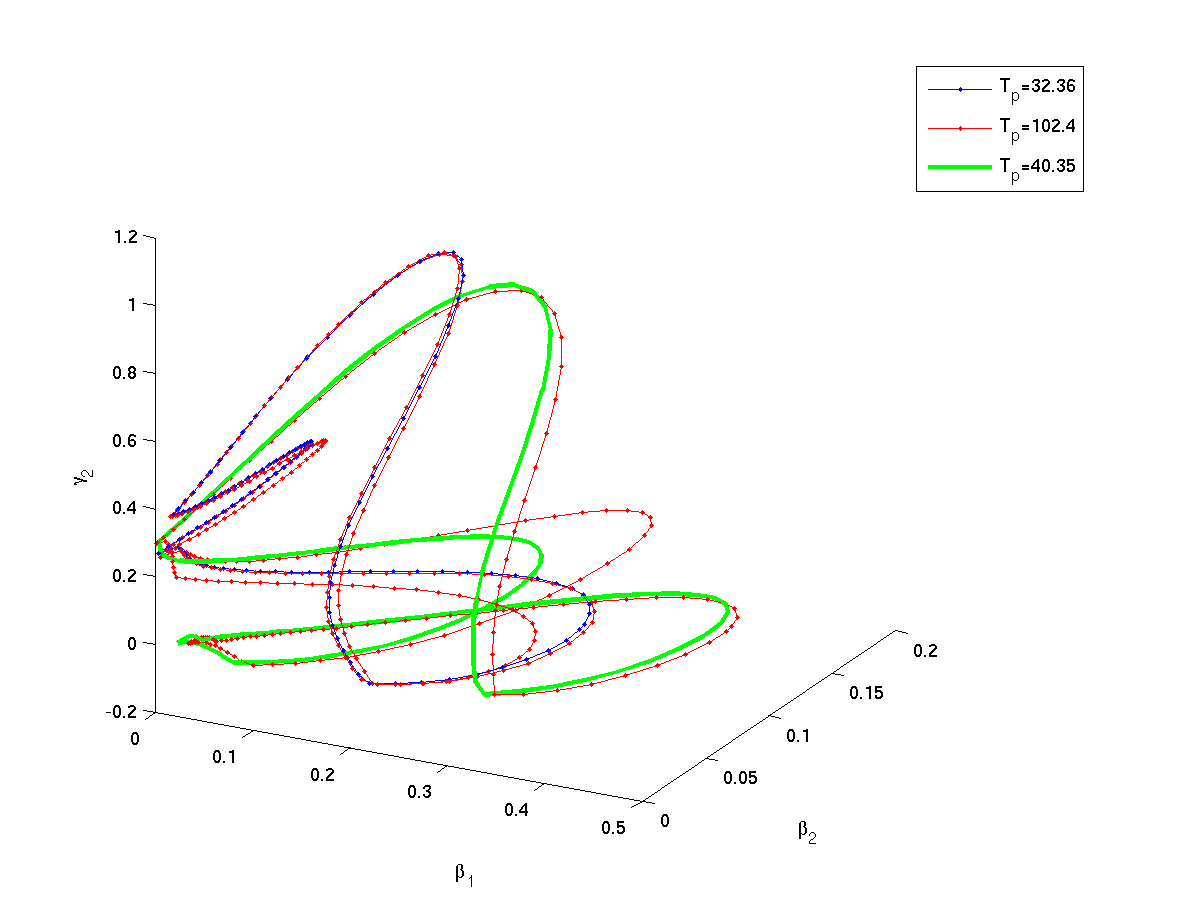
\includegraphics[width=0.45\textwidth]{ks22ppoT10235shad.png}~
    (b)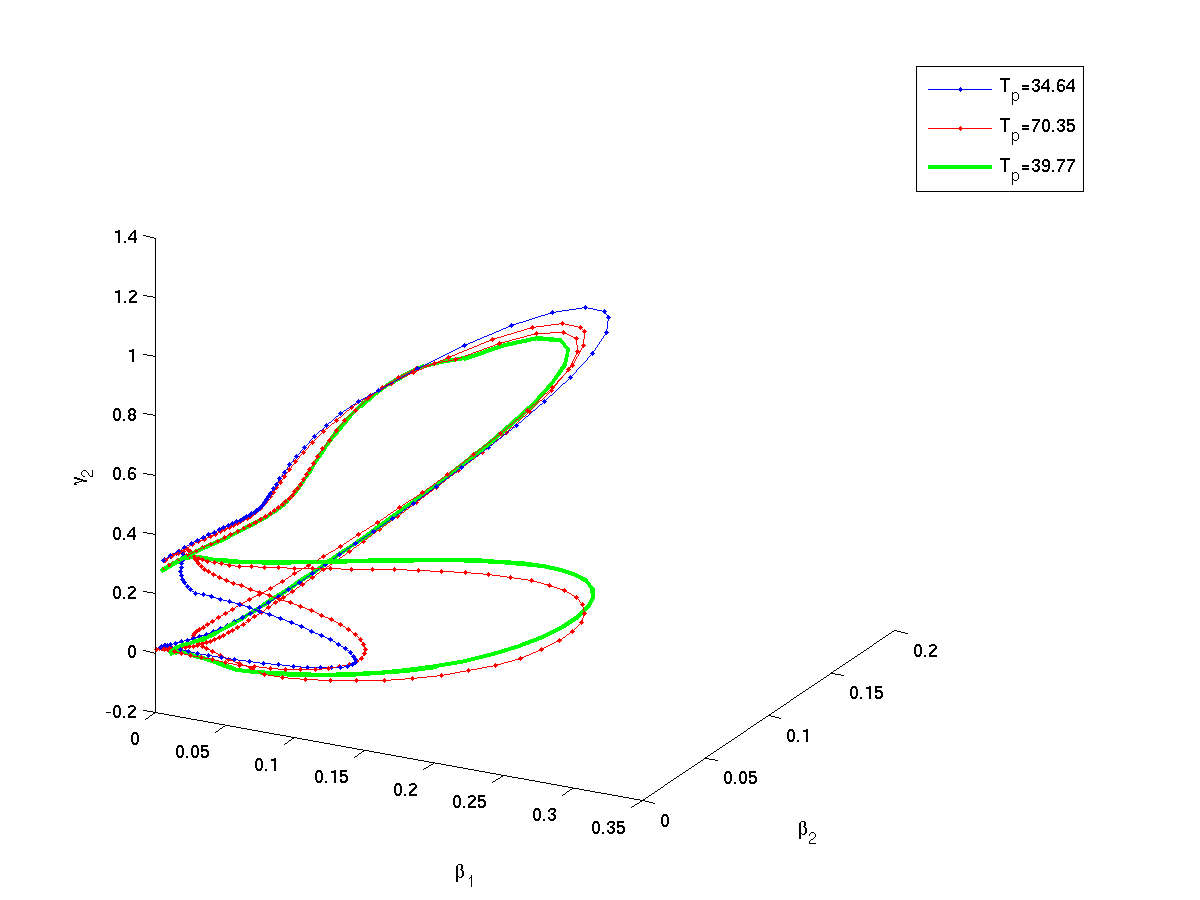
\includegraphics[width=0.45\textwidth]{ks22ppoT7035shad.png}\\
    (c)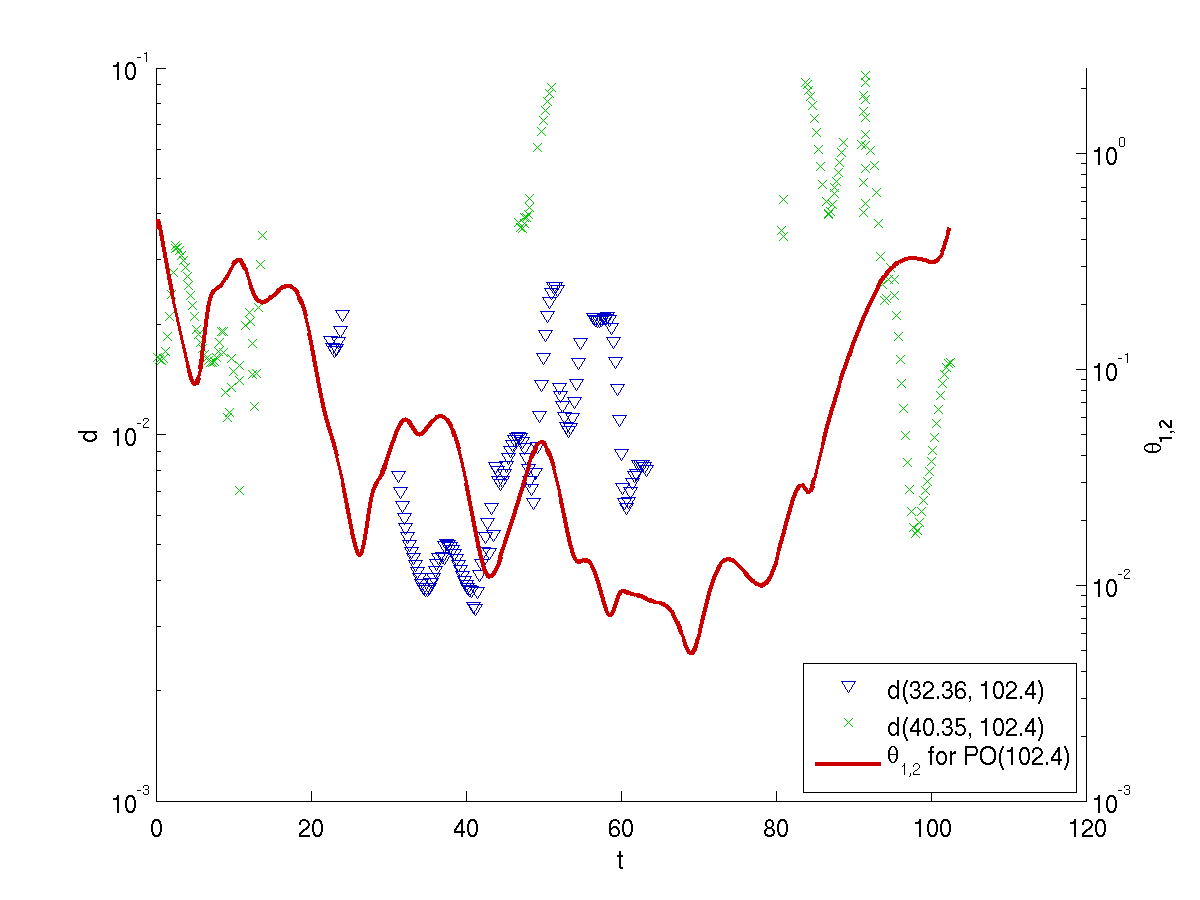
\includegraphics[width=0.45\textwidth]{ks22ppoT10235angl_dist.png}~
    (d)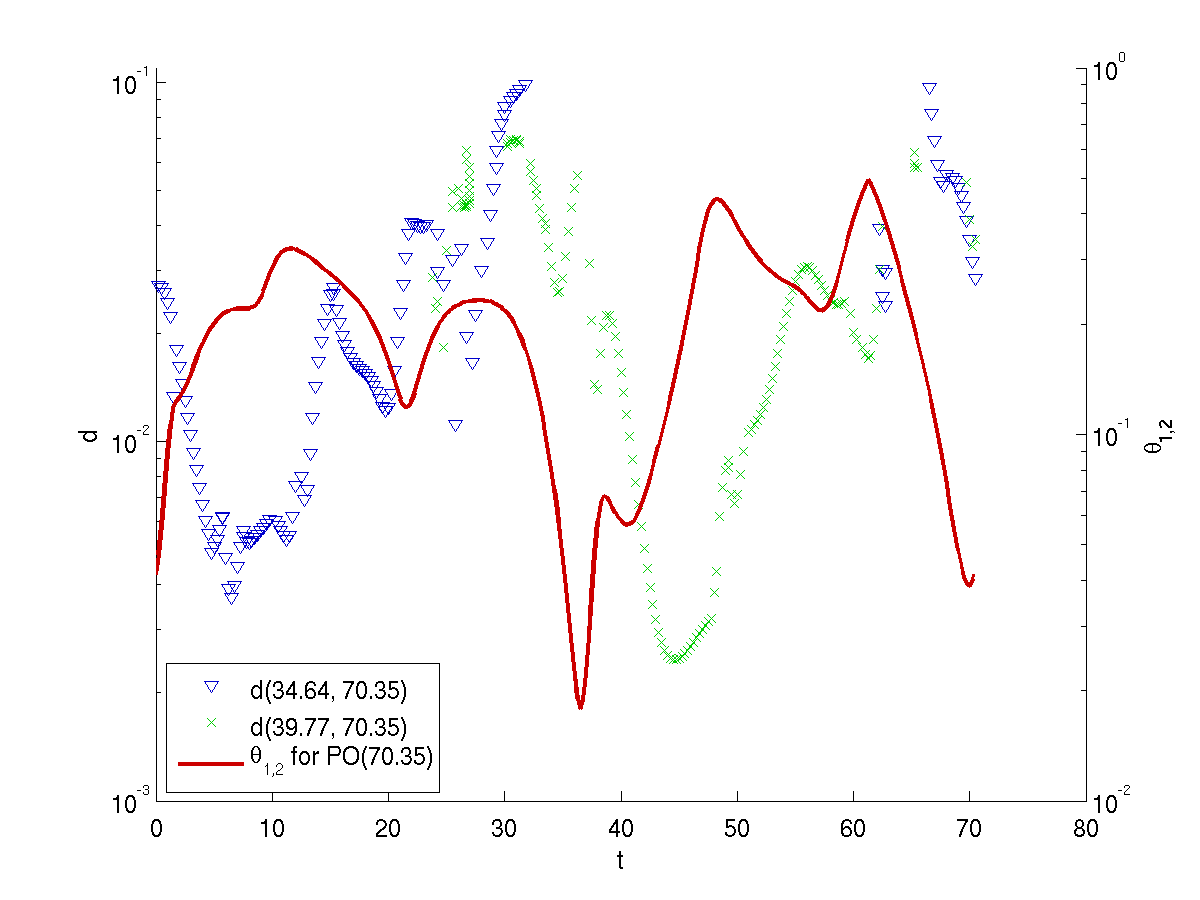
\includegraphics[width=0.45\textwidth]{ks22ppoT7035angl_dist.png}
  \end{center}
  \caption{Shadowing of periodic orbits. (a) Hyperbolic pre-periodic orbits
    \PO{32.36} and \PO{40.35} shadow \PO{102.4} which appears to be close
    to non-hyperbolicity. Note that \PO{102.4} traces \PO{32.36} twice.
    (b) \PO{70.35}, is shadowed by \RPO{34.64} and \RPO{39.77}.
    (c) Angle of first two Floquet eigenvectors along \PO{102.4} (red, solid line) and
    closest distance from \PO{102.4} of points on \PO{32.36} (blue triangles) and \PO{40.35}
    (green crosses). (d) Angle of first two Floquet eigenvectors along \PO{70.45} (red, solid line) and
    closest distance from \RPO{70.45} of points on \PO{34.64} (blue triangles) and \RPO{39.77}
    (green crosses).
    }
  \label{fig:ks22shad}
\end{figure}

\begin{table}[h!]
\caption{ Period $T_p$, shift $\shift_p$, leading (non marginal) Floquer multipliers $\ExpaEig_{p,i}$,
	  corresponding exponents $\eigRe[p, i]$ and minimum angle of first two (non marginal) Floquet
	  eigenvectors for each orbit.	
        }\label{tab:ks22shad}
\begin{center}
\begin{tabular}{ccccrrc}
    $T_p$  & $\shift_p$  & $\ExpaEig_{p,1}$ & $\ExpaEig_{p,2}$ & \eigRe[p, 1] & \eigRe[p, 2] & $\theta_{1,2}/\pi$  \\\hline
     32.36 &-- &  $-45.4\pm 47.9i$ & $1.19\times 10^{-5}$  &  0.0647 &  -0.1751 & 0.1 \\
     40.35 &-- &  $1.12\times 10^8$ & $2.34\times 10^{-3}$ &  0.2297 &  -0.0750 &  0.1\\
     102.4 &-- &  $1.29\times 10^9$ & $6.10\times 10^4$  &  0.1025 &   0.0538 & 0.005\\\hline
     34.64 & 9.600 & 35.8 & 31.6  &   0.0516  &  0.0498  & -- \\
     39.77 & 1.611 & $2.73\times 10^4$ & 0.441 & 0.128 &  -0.0103 & --\\
     70.35 & -- & $2.61\times 10^4$ & $3.51\times 10^2$ & 0.0742 &   0.0417 & 0.02\\\hline
     38.66 &-- & $2.36\times 10^3$ & $4.96$ & & & 0.01
\end{tabular}
\end{center}
\end{table}

In order to find such close encounters efficiently I first tried some
rudimentary slicing but encountered problems with jumps as described
elsewhere\rf{SiCvi10,FrCv11}. So I've settled with using $\On{2}$-invariant
variables similar in spirit to the ones in my thesis\rf{SiminosThesis}
but given in a compact form without the use of computer algebra. I've noted
down the expressions in siminos/ksReduced, in case you would like to know what
is plotted in \reffig{fig:ks22shad}. I also suggest using these transformations
when looking for close encounters of chaotic trajectories with periodic orbits.

I now intent to turn to the actual computation of the angle of the difference
vector and the subspace spanned by the $n$ first Floquet eigenvectors. However,
I think I cannot get more than 6 (including marginal) eigenvectors accurately
enough to draw safe conclusions. If I am correct, then the only option would be
to send to Kazz some initial conditions for periodic orbits which come close
to a reference orbit, so that he can get the vectors with better accuracy.

Kazz, I'd also like to send you initial condition for \PO{38.66} anyway, to
see if you can verify the angle between Floquet eigenvectors being small.

%\item[2011-11-07 Kazz] Regarding svn, I have the updated source files,
%but I cannot compile the tex. It seems that many latex style files are missing.
%I found them by myself, but it doesn't work probably because of the version mismatch...
%
%\item[2011-11-07 Evangelos] No can help... sorry. I haven't used Windows for
%anything serious for too many years. Maybe Predrag knows?
%
% Predrag helped fixed this, OK now.

\item[2011-11-9 Evangelos] Note updated \reffig{fig:ks22shad} and \reftab{tab:ks22shad}.

\item[2011-11-9 Evangelos] There seems to be an unstable manifold variability argument
emerging from \reffig{fig:ks22shad} and \reftab{tab:ks22shad}. Periodic orbits
\PO{32.36} and \PO{40.35} are hyperbolic with unstable manifolds of dimension $1$ and $2$
respectively. They appear to shadow \PO{102.4} which has a $2-$dimensional unstable manifold
and small minimum angle of the two unstable eigenvectors, \ie\ it would appear
to be non-hyperbolic. In the same manner, \RPO{34.64} and \RPO{39.77} with unstable manifolds
of dimension $1$ and $2$, respectively, shadow \PO{70.35}, which has $2$-dimensional
unstable manifold and is non-hyperbolic (I haven't computed minimum angle of eigenvectors
for \rpo s yet).

Note that \PO{38.66}(not plotted) shadows \RPO{34.64}. It would be interesting to look
at this from a (dynamical) symmetry breaking bifurcation perspective.

\item[2011-11-9 Evangelos]  In all cases shown here,
the periods of the shorter cycles (multiplied by the number of times a cycle is revisited)
(approximately) add up to the period of the longer cycle shadowed by the short ones.
I don't know whether we should read too much into \rpo\ shifts adding up to zero (or $L/2$)
when two \rpo s shadow a \po.

\item[2011-11-07 Hugues] The data of \reffig{fig:ks22shad} would be nice,
but what we would need also are the full coordinates of some selected orbits with:
\begin{itemize}
 \item not-so-large period
 \item very small minimum angle
 \item preferably first Floquet exponent near the first Lyapunov exponent
\end{itemize}

 From \reffig{fig:ks22shad}, we can see that there are certainly some like
that with a period near 80, and probably some not so bad with period around 40...


\item[2011-11-9 Evangelos] I think the two longer orbits in
\reftab{tab:ks22shad} are good candidates (although Floquet exponent is
not very close to the first Lyapunov exponent) for Kazz to repeat the
calculations in his draft. I will study them in more detail anyway, to
see where the angle of eigenvectors becomes minimal, \etc.

\item[2011-11-15 Evangelos] Updated \reffig{fig:ks22shad}. For each of
the numerically computed points along each of the shorter cycles we plot
the minimum distance from any of the numerically computed points along
the longer cycle to which they come close. We also plot the angle
$\theta_{1,2}$ of the unstable Floquet eigenvectors along the points of
the longer cycle. For both cases shown in \reffig{fig:ks22shad}, we
observe that (local) minima of $\theta_{1,2}$ are associated with passage
from the neighborhood of one of the shorter cycles to the neighborhood of
the other. For instance, in \reffig{fig:ks22shad}(d) we can see that
points on \PO{70.45} which are close to \RPO{34.64} are separated by
points close to \RPO{39.77} by the global minimum of $\theta_{1,2}$ at
$t\simeq37$, while a local minimum at $t\simeq70$ is associated to
passage from the neighborhood of \RPO{39.77} to that of \RPO{34.64}.

\item[2011-11-15 Predrag] (a very minor suggestion) - I guess your angle
is always positive, so why not plot $(t,\ln \theta_{1,2}(t))$ - it will
emphasize the close passages, which is what you care about.

\item[2011-11-16 Evangelos] Both distances and angles are already plotted
in logarithmic scale to emphasize close passages. 

\item[2011-11-15 Predrag] (Less minor:) sooner or later you have to bite
a bullet and start looking at the periodic points and their unstable
manifolds in sets of Poincar\'e sections defined at well chosen template
points. \refFig{fig:ks22shad} quickly becomes a meaningless jumble (that
is Gibson insists doing with our \pCf\ \po s, and nothing can be
understood this way). I'm fairly convinced that siminos/ksReduced
approach will not work for high-dimensional flows (it is no different
from using low Fourier modes to capture highly turbulent states), but
I'll shut up - if you make it work for \KS, I'll be impressed.

\item[2011-11-16 Evangelos] The scope of siminos/ksReduced would be to
demonstrate symmetry reduction, not to reduce \KS\ flow to return maps.
The latter would be left to some subsequent paper and indeed someone will have
to bite a bullet and do what you suggest (maybe this will be me anyway). 

`` It is no different from using low Fourier modes to capture 
highly turbulent states.'' I disagree. \refFig{fig:ks22shad}(a)
and (b) indeed focus on low Fourier modes but they are just a visual aid,
not really needed here. On the other hand distance in 
\reffig{fig:ks22shad}(c) and (d) is computed in invariant variables using
\emph{all} Fourier modes (\ie\ as many as you need for a well resolved
simulation). For the Lyapunov project \reffig{fig:ks22shad}(c) and (d) 
and \reftab{tab:ks22shad} are, I think, good starting points to formulate
a conjecture.

Ideally, siminos/ksReduced would include:
\begin{itemize}
 \item some visualizations of unstable manifolds of \eqva\ and \reqva\ 
	in invariant variables, projected on local coordinate systems 
	given by the least stable eigenvectors as in our 
	SIADS paper \refref{SCD07},
 \item some visualizations illustrating how (relative) periodic orbits are
	organized by such unstable manifolds (corroborated by measuring distance
	of points on the cycles from points on the unstable manifolds),
 \item some rudimentary organization of short cycles into families using
	their mutual distance as criterion.
\end{itemize}

At this stage I don't see anything wrong with publishing a paper that does 
not tell the whole \KS\ story (even achieving 2 out of 3 goals above is a lot
of work and even writing down the symmetry invariant variables required a lot
of thinking). 

\end{description}
